% Options for packages loaded elsewhere
\PassOptionsToPackage{unicode}{hyperref}
\PassOptionsToPackage{hyphens}{url}
%
\documentclass[
]{article}
\usepackage{lmodern}
\usepackage{amssymb,amsmath}
\usepackage{ifxetex,ifluatex}
\ifnum 0\ifxetex 1\fi\ifluatex 1\fi=0 % if pdftex
  \usepackage[T1]{fontenc}
  \usepackage[utf8]{inputenc}
  \usepackage{textcomp} % provide euro and other symbols
\else % if luatex or xetex
  \usepackage{unicode-math}
  \defaultfontfeatures{Scale=MatchLowercase}
  \defaultfontfeatures[\rmfamily]{Ligatures=TeX,Scale=1}
\fi
% Use upquote if available, for straight quotes in verbatim environments
\IfFileExists{upquote.sty}{\usepackage{upquote}}{}
\IfFileExists{microtype.sty}{% use microtype if available
  \usepackage[]{microtype}
  \UseMicrotypeSet[protrusion]{basicmath} % disable protrusion for tt fonts
}{}
\makeatletter
\@ifundefined{KOMAClassName}{% if non-KOMA class
  \IfFileExists{parskip.sty}{%
    \usepackage{parskip}
  }{% else
    \setlength{\parindent}{0pt}
    \setlength{\parskip}{6pt plus 2pt minus 1pt}}
}{% if KOMA class
  \KOMAoptions{parskip=half}}
\makeatother
\usepackage{xcolor}
\IfFileExists{xurl.sty}{\usepackage{xurl}}{} % add URL line breaks if available
\IfFileExists{bookmark.sty}{\usepackage{bookmark}}{\usepackage{hyperref}}
\hypersetup{
  pdftitle={Verteilungen},
  hidelinks,
  pdfcreator={LaTeX via pandoc}}
\urlstyle{same} % disable monospaced font for URLs
\usepackage[margin=0.5cm]{geometry}
\usepackage{color}
\usepackage{fancyvrb}
\newcommand{\VerbBar}{|}
\newcommand{\VERB}{\Verb[commandchars=\\\{\}]}
\DefineVerbatimEnvironment{Highlighting}{Verbatim}{commandchars=\\\{\}}
% Add ',fontsize=\small' for more characters per line
\usepackage{framed}
\definecolor{shadecolor}{RGB}{248,248,248}
\newenvironment{Shaded}{\begin{snugshade}}{\end{snugshade}}
\newcommand{\AlertTok}[1]{\textcolor[rgb]{0.94,0.16,0.16}{#1}}
\newcommand{\AnnotationTok}[1]{\textcolor[rgb]{0.56,0.35,0.01}{\textbf{\textit{#1}}}}
\newcommand{\AttributeTok}[1]{\textcolor[rgb]{0.77,0.63,0.00}{#1}}
\newcommand{\BaseNTok}[1]{\textcolor[rgb]{0.00,0.00,0.81}{#1}}
\newcommand{\BuiltInTok}[1]{#1}
\newcommand{\CharTok}[1]{\textcolor[rgb]{0.31,0.60,0.02}{#1}}
\newcommand{\CommentTok}[1]{\textcolor[rgb]{0.56,0.35,0.01}{\textit{#1}}}
\newcommand{\CommentVarTok}[1]{\textcolor[rgb]{0.56,0.35,0.01}{\textbf{\textit{#1}}}}
\newcommand{\ConstantTok}[1]{\textcolor[rgb]{0.00,0.00,0.00}{#1}}
\newcommand{\ControlFlowTok}[1]{\textcolor[rgb]{0.13,0.29,0.53}{\textbf{#1}}}
\newcommand{\DataTypeTok}[1]{\textcolor[rgb]{0.13,0.29,0.53}{#1}}
\newcommand{\DecValTok}[1]{\textcolor[rgb]{0.00,0.00,0.81}{#1}}
\newcommand{\DocumentationTok}[1]{\textcolor[rgb]{0.56,0.35,0.01}{\textbf{\textit{#1}}}}
\newcommand{\ErrorTok}[1]{\textcolor[rgb]{0.64,0.00,0.00}{\textbf{#1}}}
\newcommand{\ExtensionTok}[1]{#1}
\newcommand{\FloatTok}[1]{\textcolor[rgb]{0.00,0.00,0.81}{#1}}
\newcommand{\FunctionTok}[1]{\textcolor[rgb]{0.00,0.00,0.00}{#1}}
\newcommand{\ImportTok}[1]{#1}
\newcommand{\InformationTok}[1]{\textcolor[rgb]{0.56,0.35,0.01}{\textbf{\textit{#1}}}}
\newcommand{\KeywordTok}[1]{\textcolor[rgb]{0.13,0.29,0.53}{\textbf{#1}}}
\newcommand{\NormalTok}[1]{#1}
\newcommand{\OperatorTok}[1]{\textcolor[rgb]{0.81,0.36,0.00}{\textbf{#1}}}
\newcommand{\OtherTok}[1]{\textcolor[rgb]{0.56,0.35,0.01}{#1}}
\newcommand{\PreprocessorTok}[1]{\textcolor[rgb]{0.56,0.35,0.01}{\textit{#1}}}
\newcommand{\RegionMarkerTok}[1]{#1}
\newcommand{\SpecialCharTok}[1]{\textcolor[rgb]{0.00,0.00,0.00}{#1}}
\newcommand{\SpecialStringTok}[1]{\textcolor[rgb]{0.31,0.60,0.02}{#1}}
\newcommand{\StringTok}[1]{\textcolor[rgb]{0.31,0.60,0.02}{#1}}
\newcommand{\VariableTok}[1]{\textcolor[rgb]{0.00,0.00,0.00}{#1}}
\newcommand{\VerbatimStringTok}[1]{\textcolor[rgb]{0.31,0.60,0.02}{#1}}
\newcommand{\WarningTok}[1]{\textcolor[rgb]{0.56,0.35,0.01}{\textbf{\textit{#1}}}}
\usepackage{graphicx,grffile}
\makeatletter
\def\maxwidth{\ifdim\Gin@nat@width>\linewidth\linewidth\else\Gin@nat@width\fi}
\def\maxheight{\ifdim\Gin@nat@height>\textheight\textheight\else\Gin@nat@height\fi}
\makeatother
% Scale images if necessary, so that they will not overflow the page
% margins by default, and it is still possible to overwrite the defaults
% using explicit options in \includegraphics[width, height, ...]{}
\setkeys{Gin}{width=\maxwidth,height=\maxheight,keepaspectratio}
% Set default figure placement to htbp
\makeatletter
\def\fps@figure{htbp}
\makeatother
\setlength{\emergencystretch}{3em} % prevent overfull lines
\providecommand{\tightlist}{%
  \setlength{\itemsep}{0pt}\setlength{\parskip}{0pt}}
\setcounter{secnumdepth}{-\maxdimen} % remove section numbering

\title{Verteilungen}
\author{}
\date{\vspace{-2.5em}28.03.2022}

\begin{document}
\maketitle

\hypertarget{bibliotheken-laden-hilfsfunktion}{%
\section{Bibliotheken laden,
Hilfsfunktion}\label{bibliotheken-laden-hilfsfunktion}}

\begin{Shaded}
\begin{Highlighting}[]
\KeywordTok{library}\NormalTok{(stringr)    }\CommentTok{# String-verarbeitung}
\KeywordTok{library}\NormalTok{(ggplot2)    }\CommentTok{# moderne plots}
\CommentTok{#library(gridExtra)}

\NormalTok{debug <-}\StringTok{ }\NormalTok{T  }\CommentTok{# debug printout}
\NormalTok{debug <-}\StringTok{ }\NormalTok{F  }\CommentTok{# kein debug printout}
\NormalTok{Log <-}\StringTok{ }\ControlFlowTok{function}\NormalTok{(string) \{}
  \ControlFlowTok{if}\NormalTok{(debug)\{}\KeywordTok{print}\NormalTok{(string)\}  }
\NormalTok{\}}
\end{Highlighting}
\end{Shaded}

\hypertarget{resistenzenu.csv-o.-resistenzenle8000.csv-o.resistenzengt8000.csv-einlesen}{%
\section{ResistenzenU.csv o. ResistenzenLE8000.csv
o.ResistenzenGT8000.csv
einlesen}\label{resistenzenu.csv-o.-resistenzenle8000.csv-o.resistenzengt8000.csv-einlesen}}

Diese Tabellen wurden von Resistenzen.Rmd erzeugt. Sie evtl. auch
ansehen

\begin{Shaded}
\begin{Highlighting}[]
\NormalTok{Schicht <-}\StringTok{ "U"}
\NormalTok{Schicht <-}\StringTok{ "LE8000"}
\NormalTok{Schicht <-}\StringTok{ "GT8000"}

\NormalTok{Resistenzen <-}\StringTok{ }\KeywordTok{read.csv}\NormalTok{(}\KeywordTok{paste}\NormalTok{(}\StringTok{"Resistenzen"}\NormalTok{,Schicht,}\StringTok{".csv"}\NormalTok{,}\DataTypeTok{sep=}\StringTok{""}\NormalTok{))}

\CommentTok{# csv raussschreiben u. wieder einlesen fügt vorne Index-Spalte an; diese entfernen :}
\NormalTok{Resistenzen[,}\DecValTok{1}\NormalTok{] <-}\StringTok{ }\OtherTok{NULL}                      

\ControlFlowTok{if}\NormalTok{(debug)\{}\KeywordTok{View}\NormalTok{(Resistenzen)\}}
\end{Highlighting}
\end{Shaded}

\hypertarget{verteilungen}{%
\subsection{Verteilungen}\label{verteilungen}}

\begin{Shaded}
\begin{Highlighting}[]
\CommentTok{# Hilfs-Dataframes, implizit sollte genügen!}

\NormalTok{ResistenzenWM1  <-}\StringTok{ }\NormalTok{Resistenzen[Resistenzen[}\StringTok{"WM.group"}\NormalTok{]  }\OperatorTok{==}\StringTok{ "1"}\NormalTok{,]  }\CommentTok{#    waste milk Group}
\NormalTok{ResistenzenWM2  <-}\StringTok{ }\NormalTok{Resistenzen[Resistenzen[}\StringTok{"WM.group"}\NormalTok{ ] }\OperatorTok{==}\StringTok{ "2"}\NormalTok{,]  }\CommentTok{# no waste milk Group}
\CommentTok{#if(debug)\{View(ResistenzenWM2)\}}

\NormalTok{ResistenzenOLS0 <-}\StringTok{ }\NormalTok{Resistenzen[Resistenzen[}\StringTok{"OLS.group"}\NormalTok{] }\OperatorTok{==}\StringTok{ "0"}\NormalTok{,]  }\CommentTok{#    other livestock Group}
\NormalTok{ResistenzenOLS1 <-}\StringTok{ }\NormalTok{Resistenzen[Resistenzen[}\StringTok{"OLS.group"}\NormalTok{] }\OperatorTok{==}\StringTok{ "1"}\NormalTok{,]  }\CommentTok{# no other livestock  Group}
\CommentTok{#if(debug)\{View(ResistenzenOLS0);View(ResistenzenOLS1)\}}

\NormalTok{ResistenzenIAC0 <-}\StringTok{ }\NormalTok{Resistenzen[Resistenzen[}\StringTok{"IAC.group"}\NormalTok{] }\OperatorTok{==}\StringTok{ "0"}\NormalTok{,]  }\CommentTok{#    ill animals in calving box Group}
\NormalTok{ResistenzenIAC1 <-}\StringTok{ }\NormalTok{Resistenzen[Resistenzen[}\StringTok{"IAC.group"}\NormalTok{] }\OperatorTok{==}\StringTok{ "1"}\NormalTok{,]  }\CommentTok{# no ill animals in calving box Group}
\CommentTok{#if(debug)\{View(ResistenzenIAC0);View(ResistenzenIAC1)\}}

\NormalTok{ResistenzenHSC0 <-}\StringTok{ }\NormalTok{Resistenzen[Resistenzen[}\StringTok{"HSC.group"}\NormalTok{] }\OperatorTok{==}\StringTok{ "0"}\NormalTok{,]  }\CommentTok{# stable w\textbackslash{}o  outlet}
\NormalTok{ResistenzenHSC1 <-}\StringTok{ }\NormalTok{Resistenzen[Resistenzen[}\StringTok{"HSC.group"}\NormalTok{] }\OperatorTok{==}\StringTok{ "1"}\NormalTok{,]  }\CommentTok{# stable with outlet}
\NormalTok{ResistenzenHSC2 <-}\StringTok{ }\NormalTok{Resistenzen[Resistenzen[}\StringTok{"HSC.group"}\NormalTok{] }\OperatorTok{==}\StringTok{ "2"}\NormalTok{,]  }\CommentTok{# outdoors}
\NormalTok{ResistenzenHSC3 <-}\StringTok{ }\NormalTok{Resistenzen[Resistenzen[}\StringTok{"HSC.group"}\NormalTok{] }\OperatorTok{==}\StringTok{ "3"}\NormalTok{,]  }\CommentTok{# 0+1}
\NormalTok{ResistenzenHSC4 <-}\StringTok{ }\NormalTok{Resistenzen[Resistenzen[}\StringTok{"HSC.group"}\NormalTok{] }\OperatorTok{==}\StringTok{ "4"}\NormalTok{,]  }\CommentTok{# 1+2}
\NormalTok{ResistenzenHSC5 <-}\StringTok{ }\NormalTok{Resistenzen[Resistenzen[}\StringTok{"HSC.group"}\NormalTok{] }\OperatorTok{==}\StringTok{ "5"}\NormalTok{,]  }\CommentTok{# 0+2}
\CommentTok{#if(debug)\{View(ResistenzenHSC0);View(ResistenzenHSC1);View(ResistenzenHSC2);View(ResistenzenHSC3);View(ResistenzenHSC4);View(ResistenzenHSC5)\}}
\end{Highlighting}
\end{Shaded}

Graphiken und Deskriptive Analyse: Für diesen Fall analysieren wir die
(meist links und/oder rechts abgeschnittenen) Verteilungen

\begin{Shaded}
\begin{Highlighting}[]
\NormalTok{graphisch <-}\StringTok{ }\ControlFlowTok{function}\NormalTok{(groups,antib, anfang,ende, schrittBin,schrittLab) \{    }

  \ControlFlowTok{if}\NormalTok{ (ende }\OperatorTok{<}\StringTok{ }\DecValTok{0}\NormalTok{) \{            }\CommentTok{# kleiner Trick um zusätzliches Funktionsargument zu vermeiden}
\NormalTok{    Ende=F}
\NormalTok{    ende =}\StringTok{ }\OperatorTok{-}\NormalTok{ende}
\NormalTok{  \} }\ControlFlowTok{else}\NormalTok{\{}
\NormalTok{    Ende=T}
\NormalTok{  \}}
  \KeywordTok{Log}\NormalTok{(}\KeywordTok{paste}\NormalTok{(}\StringTok{"Ende, ende ="}\NormalTok{,Ende,ende))}
  
  \KeywordTok{dir.create}\NormalTok{(}\KeywordTok{paste}\NormalTok{(}\StringTok{"verteilungen_"}\NormalTok{,Schicht,}\DataTypeTok{sep=}\StringTok{""}\NormalTok{))             }\CommentTok{# directory for writing the plots}
  
  \ControlFlowTok{if}\NormalTok{(groups }\OperatorTok{==}\StringTok{ "WM.group"}\NormalTok{ )\{}
\NormalTok{    listdfs <-}\StringTok{ }\KeywordTok{list}\NormalTok{(Resistenzen    , ResistenzenWM1 , ResistenzenWM2 )  }\CommentTok{#  implizit sollte genügen! (Vektor klappt hier nicht)}
\NormalTok{    Titel   <-}\StringTok{ }\KeywordTok{c}\NormalTok{(   }\StringTok{"WM or not"}\NormalTok{, }\StringTok{"WM           "}\NormalTok{, }\StringTok{"no WM     "}\NormalTok{)}
\NormalTok{  \}}
   \ControlFlowTok{if}\NormalTok{(groups }\OperatorTok{==}\StringTok{ "OLS.group"}\NormalTok{ )\{}
\NormalTok{    listdfs <-}\StringTok{ }\KeywordTok{list}\NormalTok{(Resistenzen    , ResistenzenOLS1 , ResistenzenOLS0 )  }
\NormalTok{    Titel   <-}\StringTok{ }\KeywordTok{c}\NormalTok{(   }\StringTok{"OLS or not"}\NormalTok{, }\StringTok{"OLS           "}\NormalTok{, }\StringTok{"no OLS      "}\NormalTok{)}
\NormalTok{  \}}
   \ControlFlowTok{if}\NormalTok{(groups }\OperatorTok{==}\StringTok{ "IAC.group"}\NormalTok{ )\{}
\NormalTok{    listdfs <-}\StringTok{ }\KeywordTok{list}\NormalTok{(Resistenzen    , ResistenzenIAC1 , ResistenzenIAC0 ) }
\NormalTok{    Titel   <-}\StringTok{ }\KeywordTok{c}\NormalTok{(   }\StringTok{"IAC or not"}\NormalTok{, }\StringTok{"IAC           "}\NormalTok{, }\StringTok{"no IAC      "}\NormalTok{)}
\NormalTok{  \}}
  \ControlFlowTok{if}\NormalTok{(groups }\OperatorTok{==}\StringTok{ "HSC.group"}\NormalTok{)\{}
\NormalTok{    listdfs <-}\StringTok{ }\KeywordTok{list}\NormalTok{(Resistenzen    , ResistenzenHSC0, ResistenzenHSC1, }
\NormalTok{                    ResistenzenHSC2, ResistenzenHSC3, ResistenzenHSC4, ResistenzenHSC5)  }
\NormalTok{    Titel   <-}\StringTok{ }\KeywordTok{c}\NormalTok{(   }\StringTok{"arbitrary HSC          "}\NormalTok{, }
                    \StringTok{"0: stable w}\CharTok{\textbackslash{}\textbackslash{}}\StringTok{o  outlet"}\NormalTok{, }\StringTok{"1: stable with outlet"}\NormalTok{, }\StringTok{"2: outdoors          "}\NormalTok{,}\StringTok{"0+1                  "}\NormalTok{,}\StringTok{"1+2                  "}\NormalTok{,}\StringTok{"0+2                  "}\NormalTok{)}
\NormalTok{  \}}
  
  \ControlFlowTok{for}\NormalTok{ (i }\ControlFlowTok{in} \DecValTok{2}\OperatorTok{:}\KeywordTok{length}\NormalTok{(Titel))\{     }\CommentTok{# nicht 1. plot "XY oder nicht"  deskriptive Statistik - geht sicher o. eigene DFs!!? }
\NormalTok{    DF <-}\StringTok{ }\NormalTok{listdfs[[i]]            }\CommentTok{# listdfs kürzer: nur hier explizit?}
    
\NormalTok{    numstrings <-}\StringTok{ }\KeywordTok{str_replace}\NormalTok{(DF[[antib]], }\KeywordTok{paste0}\NormalTok{(}\StringTok{"<="}\NormalTok{,anfang),  }\KeywordTok{as.character}\NormalTok{(anfang))  }
    \CommentTok{# z.B. "1" als numerischer Platzhalter für "<=1" }
\NormalTok{    numstrings <-}\StringTok{ }\KeywordTok{str_replace}\NormalTok{(numstrings          , }\KeywordTok{paste0}\NormalTok{(}\StringTok{">"}\NormalTok{,ende)   , }\KeywordTok{as.character}\NormalTok{(ende)) }\CommentTok{#+1))   }
    \CommentTok{# z.B. "33" als numerischer Platzhalter für ">32"}
\NormalTok{    numbers <-}\StringTok{ }\KeywordTok{as.numeric}\NormalTok{(numstrings )      }\CommentTok{# jetzt alles als Zahlen                                                       }

    \KeywordTok{Log}\NormalTok{(}\StringTok{"numbers ="}\NormalTok{);}\KeywordTok{Log}\NormalTok{(numbers)}
    \CommentTok{# Median könnte im "<=" Bereich liegen oder im ">=", entsprechend reagieren:}
\NormalTok{    median <-}\StringTok{ }\KeywordTok{median}\NormalTok{(numbers, }\DataTypeTok{na.rm=}\NormalTok{T)  }\CommentTok{# (na.rm=T fürs Lesen aus file, vorher war das "NA")}
\NormalTok{    rel <-}\StringTok{ "="}                          \CommentTok{# Relations-Symbol}
    \KeywordTok{Log}\NormalTok{(}\KeywordTok{paste}\NormalTok{( }\StringTok{"median, anfang ="}\NormalTok{,median, anfang ))}
    \ControlFlowTok{if}\NormalTok{(median }\OperatorTok{==}\StringTok{ }\NormalTok{anfang)\{}
\NormalTok{      rel <-}\StringTok{ "<="} 
\NormalTok{    \} }
    \ControlFlowTok{if}\NormalTok{(Ende }\OperatorTok{&&}\StringTok{ }\NormalTok{median }\OperatorTok{==}\StringTok{ }\NormalTok{ende)\{}
\NormalTok{      rel <-}\StringTok{ ">"}
\NormalTok{    \} }

    \KeywordTok{print}\NormalTok{(}\KeywordTok{paste}\NormalTok{(antib,}\StringTok{"- Resistance,"}\NormalTok{, Titel[i], }\StringTok{":"}\NormalTok{))}
    \KeywordTok{print}\NormalTok{(}\KeywordTok{paste}\NormalTok{(}\StringTok{"  Median            "}\NormalTok{, rel, median))}
    
    \ControlFlowTok{if}\NormalTok{(Ende }\OperatorTok{&&}\StringTok{ }\NormalTok{(}\KeywordTok{max}\NormalTok{(numbers, }\DataTypeTok{na.rm=}\NormalTok{T) }\OperatorTok{>}\StringTok{ }\NormalTok{ende))\{  }\CommentTok{# gibt overflow bin, ist nicht leer: Verteilung nicht nach oben beschränkt}
                                                            
      \CommentTok{# kleinste Werte kleinstmöglich und grösste Werte kleinstmöglich ergibt Mindestwert des Mittelwertes}
\NormalTok{      mean <-}\StringTok{ }\KeywordTok{mean}\NormalTok{(}\KeywordTok{replace}\NormalTok{(numbers, numbers}\OperatorTok{==}\NormalTok{anfang, }\DecValTok{0}\NormalTok{), }\DataTypeTok{na.rm=}\NormalTok{T)    }
                                
      \KeywordTok{print}\NormalTok{(}\KeywordTok{paste}\NormalTok{(}\StringTok{"  Mean           >= "}\NormalTok{, mean  ))}
      \KeywordTok{print}\NormalTok{(}\StringTok{""}\NormalTok{)}
\NormalTok{    \} }\ControlFlowTok{else}\NormalTok{ \{                      }\CommentTok{# Verteilung nach oben beschränkt}
      \ControlFlowTok{if}\NormalTok{ (anfang }\OperatorTok\StringTok{ }\NormalTok{numbers) \{  }\CommentTok{# Verteilung nach oben beschränkt, nicht nach unten }
                                  \CommentTok{#  (underflow bin gibt's FAST immer)}
\NormalTok{        mean1 <-}\StringTok{ }\KeywordTok{mean}\NormalTok{(numbers, }\DataTypeTok{na.rm=}\NormalTok{T)    }\CommentTok{# kleinste Werte grösstmöglich gibt Höchstwert des Mittelwertes}
      
\NormalTok{        numbers0 <-}\StringTok{ }\KeywordTok{replace}\NormalTok{(numbers, numbers}\OperatorTok{==}\NormalTok{anfang, }\DecValTok{0}\NormalTok{)    }\CommentTok{# kleinste Werte kleinstmöglich }
\NormalTok{        mean0 <-}\StringTok{ }\KeywordTok{mean}\NormalTok{(numbers0, }\DataTypeTok{na.rm=}\NormalTok{T)                             }\CommentTok{#   ergibt Mindestwert des Mittelwertes}
        \KeywordTok{print}\NormalTok{(}\KeywordTok{paste}\NormalTok{(}\StringTok{"  Mean   in "}\NormalTok{, }\KeywordTok{sprintf}\NormalTok{(}\StringTok{"%.3f"}\NormalTok{,mean0), }\StringTok{"..."}\NormalTok{, }\KeywordTok{sprintf}\NormalTok{(}\StringTok{"%.3f"}\NormalTok{,mean1)  ))}
        \KeywordTok{print}\NormalTok{(}\StringTok{""}\NormalTok{)}
\NormalTok{      \} }\ControlFlowTok{else}\NormalTok{ \{                    }\CommentTok{# Verteilung nach oben und unten beschränkt : einfachster Fall}
        \KeywordTok{print}\NormalTok{(}\KeywordTok{paste}\NormalTok{(}\StringTok{"  Mean   = "}\NormalTok{, }\KeywordTok{sprintf}\NormalTok{(}\StringTok{"%.3f"}\NormalTok{,}\KeywordTok{mean}\NormalTok{(numbers, }\DataTypeTok{na.rm=}\NormalTok{T)) ) )}
        \KeywordTok{print}\NormalTok{(}\StringTok{""}\NormalTok{)}
\NormalTok{      \}}
\NormalTok{    \}}
\NormalTok{  \}}
  
\NormalTok{  DF2 <-}\StringTok{ }\NormalTok{Resistenzen }

\NormalTok{  numstrings <-}\StringTok{ }\KeywordTok{str_replace}\NormalTok{(DF2[[antib]], }\KeywordTok{paste0}\NormalTok{(}\StringTok{"<="}\NormalTok{,anfang),  }\KeywordTok{as.character}\NormalTok{(anfang))   }\CommentTok{# \textbackslash{}\textbackslash{} OBEN SCHON: factor out !! oder lieber TeilDFs implizit ??}
  \CommentTok{# z.B. "1" als numerischer Platzhalter für "<=1" }
\NormalTok{  numstrings <-}\StringTok{ }\KeywordTok{str_replace}\NormalTok{(numstrings          , }\KeywordTok{paste0}\NormalTok{(}\StringTok{">"}\NormalTok{,ende)   , }\KeywordTok{as.character}\NormalTok{(ende)) }\CommentTok{#+1))   }
  \CommentTok{# z.B. "33" als numerischer Platzhalter für ">32"}
\NormalTok{  numbers <-}\StringTok{ }\KeywordTok{as.numeric}\NormalTok{(numstrings )      }\CommentTok{# jetzt alles als Zahlen                                                       }
  \KeywordTok{Log}\NormalTok{(}\DecValTok{3}\NormalTok{)}

\NormalTok{  DF2}\OperatorTok{$}\NormalTok{numbers <-}\StringTok{ }\NormalTok{numbers}
  \KeywordTok{Log}\NormalTok{(}\StringTok{"i, numbers="}\NormalTok{);}\KeywordTok{Log}\NormalTok{(i);}\KeywordTok{Log}\NormalTok{(numbers)}

  \CommentTok{# https://stackoverflow.com/questions/23944355/r-hist-right-left-clump-binning war hier eine Inspiration,}
  \CommentTok{# fieseln für die tick labels weil R sonst aus Platzproblemen das wichtige letzte tick label unterdrückt:}
  \ControlFlowTok{if}\NormalTok{(Ende) \{}
\NormalTok{    seqAt  <-}\StringTok{ }\KeywordTok{seq}\NormalTok{(schrittBin         ,ende}\OperatorTok{+}\NormalTok{schrittBin,}\DataTypeTok{by=}\NormalTok{schrittLab)  }\CommentTok{# kleineres ende+... klappt nicht}
\NormalTok{    seqAt[}\KeywordTok{length}\NormalTok{(seqAt)]  <-}\StringTok{ }\NormalTok{seqAt[}\KeywordTok{length}\NormalTok{(seqAt)]}\OperatorTok{-}\NormalTok{schrittBin          }\CommentTok{# also zurückkorrigieren}
    \CommentTok{#seqAt  <- seq(schrittBin         ,ende+0.001,by=schrittLab) }
\NormalTok{  \} }\ControlFlowTok{else}\NormalTok{ \{}
\NormalTok{    seqAt  <-}\StringTok{ }\KeywordTok{seq}\NormalTok{(schrittBin,ende           ,}\DataTypeTok{by=}\NormalTok{schrittLab)  }\CommentTok{# 1 Bin weniger}
\NormalTok{  \}}
  \KeywordTok{Log}\NormalTok{(}\StringTok{"seqAt:"}\NormalTok{); }\KeywordTok{Log}\NormalTok{(seqAt)}
\NormalTok{  seqLab <-}\StringTok{ }\KeywordTok{seq}\NormalTok{(schrittBin}\OperatorTok{+}\NormalTok{schrittLab,ende           ,}\DataTypeTok{by=}\NormalTok{schrittLab)  }
\NormalTok{  seqLab <-}\StringTok{ }\KeywordTok{seq}\NormalTok{(schrittBin           ,ende}\OperatorTok{+}\NormalTok{schrittBin,}\DataTypeTok{by=}\NormalTok{schrittLab)  }
     
  \KeywordTok{Log}\NormalTok{(}\StringTok{"seqLab:"}\NormalTok{);}\KeywordTok{Log}\NormalTok{(seqLab)}
    
\NormalTok{  seqLab_cutR <-}\StringTok{ }\NormalTok{seqLab[}\DecValTok{1}\OperatorTok{:}\KeywordTok{length}\NormalTok{(seqLab)}\OperatorTok{-}\DecValTok{1}\NormalTok{]           }
  \KeywordTok{Log}\NormalTok{(}\StringTok{"seqLab_cutR:"}\NormalTok{);}\KeywordTok{Log}\NormalTok{(seqLab_cutR)}
    
\NormalTok{  seqLab_cutLR <-}\StringTok{ }\NormalTok{seqLab_cutR[}\DecValTok{2}\OperatorTok{:}\KeywordTok{length}\NormalTok{(seqLab_cutR)]  }\CommentTok{# ... [2:...] klappt nicht}
  \KeywordTok{Log}\NormalTok{(}\StringTok{"seqLab_cutLR:"}\NormalTok{);}\KeywordTok{Log}\NormalTok{(seqLab_cutLR)}
    
\NormalTok{  Labels <-}\StringTok{ }\KeywordTok{c}\NormalTok{(}\KeywordTok{paste0}\NormalTok{(}\StringTok{"<="}\NormalTok{,anfang),seqLab_cutLR)}
  \KeywordTok{Log}\NormalTok{(}\StringTok{"Labels, 1:"}\NormalTok{);}\KeywordTok{Log}\NormalTok{(Labels)}
    
  \ControlFlowTok{if}\NormalTok{(Ende) \{ Labels <-}\StringTok{ }\KeywordTok{c}\NormalTok{(Labels,}\KeywordTok{paste0}\NormalTok{(}\StringTok{">"}\NormalTok{,ende)) \}}
  \KeywordTok{Log}\NormalTok{(}\StringTok{"Labels, 2:"}\NormalTok{);}\KeywordTok{Log}\NormalTok{(Labels)}

  \CommentTok{#Ylab <- paste("Frequenz",antib,Titel[i])}
\NormalTok{  Ylab <-}\StringTok{ "Frequency"}
\NormalTok{  Xlab <-}\StringTok{ "Dose"}

  \KeywordTok{Log}\NormalTok{(}\StringTok{"breaks="}\NormalTok{); }\KeywordTok{Log}\NormalTok{(seqAt)}
  \KeywordTok{Log}\NormalTok{(}\StringTok{"labels ="}\NormalTok{); }\KeywordTok{Log}\NormalTok{(Labels)}
    
\NormalTok{  plot <-}\StringTok{ }\KeywordTok{ggplot}\NormalTok{(DF2, }\KeywordTok{aes}\NormalTok{(}\DataTypeTok{x=}\NormalTok{numbers)) }\OperatorTok{+}\StringTok{ }
\StringTok{    }\KeywordTok{scale_x_continuous}\NormalTok{(}\DataTypeTok{trans =} \StringTok{"log10"}\NormalTok{, }\DataTypeTok{breaks=}\NormalTok{seqAt, }\DataTypeTok{labels=}\NormalTok{Labels, }\DataTypeTok{limits=}\KeywordTok{c}\NormalTok{(anfang}\OperatorTok{*}\NormalTok{.}\DecValTok{8}\NormalTok{,ende}\OperatorTok{*}\FloatTok{1.2}\NormalTok{)) }\OperatorTok{+}\StringTok{  }
\StringTok{    }\CommentTok{# limits=anfang...ende aber bisschen mehr um dort zu plotten }
\StringTok{    }\CommentTok{# -0.01 o. *0.9; +1 o. *1.1 genügt nicht}
\StringTok{    }\KeywordTok{geom_histogram}\NormalTok{()                           }\OperatorTok{+}\StringTok{ }
\StringTok{    }\KeywordTok{theme}\NormalTok{(}\DataTypeTok{axis.text.x =} \KeywordTok{element_text}\NormalTok{(}\DataTypeTok{size=}\DecValTok{12}\NormalTok{)) }\OperatorTok{+}\StringTok{   }\CommentTok{# HSC.group kleben die labels oft aneinander}
\StringTok{    }\KeywordTok{theme}\NormalTok{(}\DataTypeTok{axis.text.y =} \KeywordTok{element_text}\NormalTok{(}\DataTypeTok{size=}\DecValTok{12}\NormalTok{)) }\OperatorTok{+}\StringTok{   }\CommentTok{# aber das ist kaum zu ändern: mit < 12 nimmt R oft noch mehr ticks!}
\StringTok{    }\KeywordTok{xlab}\NormalTok{(Xlab) }\OperatorTok{+}\StringTok{ }\KeywordTok{ylab}\NormalTok{(Ylab)                    }\OperatorTok{+}
\StringTok{    }
\StringTok{    }\KeywordTok{facet_grid}\NormalTok{(}\KeywordTok{reformulate}\NormalTok{(}\StringTok{"."}\NormalTok{,groups))    }\OperatorTok{+}\StringTok{       }\CommentTok{# vertikal   geschichtet. reformulate gibt Formel (IAC.group ~ .)  etc.}
\StringTok{    }\CommentTok{#facet_grid(reformulate(groups,"."))    +      # horizontal geschichtet - war weniger schön.}
\StringTok{    }
\StringTok{    }\KeywordTok{ggtitle}\NormalTok{(}\KeywordTok{paste}\NormalTok{(antib,}\StringTok{"for different"}\NormalTok{,groups))}
  

  \KeywordTok{print}\NormalTok{(plot)}
  \KeywordTok{ggsave}\NormalTok{(}\KeywordTok{paste}\NormalTok{(}\StringTok{"verteilungen_"}\NormalTok{,Schicht,}\StringTok{"/"}\NormalTok{, Schicht,}\StringTok{"_"}\NormalTok{,groups,}\StringTok{"_"}\NormalTok{,antib,}\StringTok{".png"}\NormalTok{, }\DataTypeTok{sep=}\StringTok{""}\NormalTok{))}

\NormalTok{\}}
\end{Highlighting}
\end{Shaded}

\hypertarget{ill-animals-in-calving-box---gruppen}{%
\subsection{Ill Animals in Calving Box -
Gruppen}\label{ill-animals-in-calving-box---gruppen}}

Mit ``IAC'' abgekürzt.

\begin{Shaded}
\begin{Highlighting}[]
  \KeywordTok{graphisch}\NormalTok{(}\StringTok{"IAC.group"}\NormalTok{, }\StringTok{"AMP"}\NormalTok{, }\DecValTok{1}\NormalTok{,}\DecValTok{32}\NormalTok{, }\DecValTok{1}\NormalTok{,}\DecValTok{8}\NormalTok{)  }
\end{Highlighting}
\end{Shaded}

\begin{verbatim}
## [1] "AMP - Resistance, IAC            :"
## [1] "  Median             = 4"
## [1] "  Mean   =  13.385"
## [1] ""
## [1] "AMP - Resistance, no IAC       :"
## [1] "  Median             = 4"
## [1] "  Mean   =  13.143"
## [1] ""
\end{verbatim}

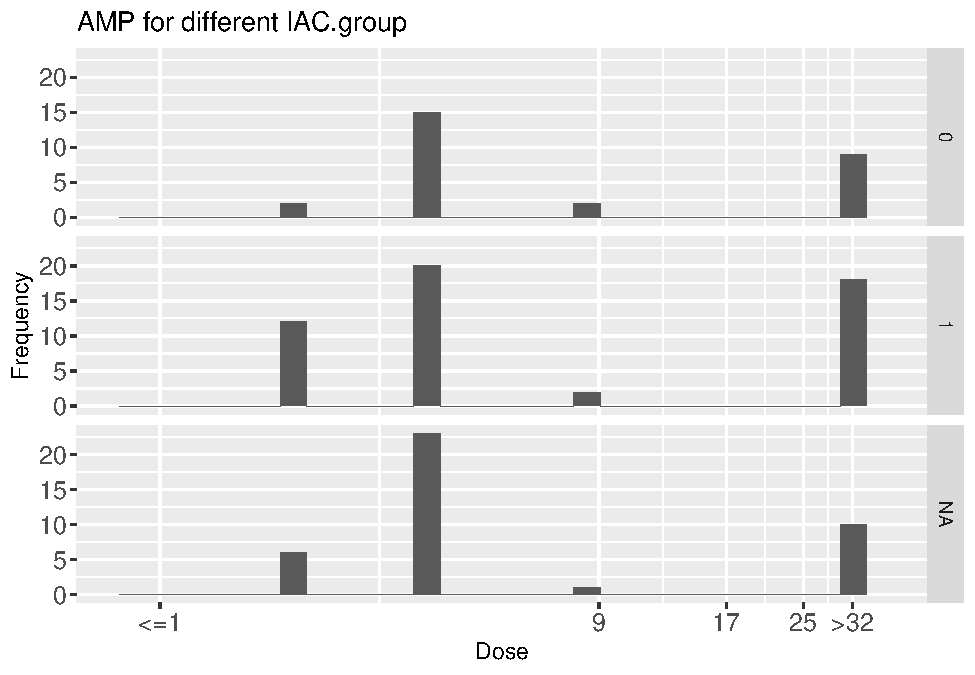
\includegraphics{Verteilungen_files/figure-latex/unnamed-chunk-5-1.pdf}

\begin{Shaded}
\begin{Highlighting}[]
  \KeywordTok{graphisch}\NormalTok{(}\StringTok{"IAC.group"}\NormalTok{, }\StringTok{"MERO"}\NormalTok{, }\FloatTok{0.03}\NormalTok{,}\OperatorTok{-}\FloatTok{0.06}\NormalTok{,   }\FloatTok{0.015}\NormalTok{,}\FloatTok{0.015}\NormalTok{ )}
\end{Highlighting}
\end{Shaded}

\begin{verbatim}
## [1] "MERO - Resistance, IAC            :"
## [1] "  Median             <= 0.03"
## [1] "  Mean   in  0.000 ... 0.030"
## [1] ""
## [1] "MERO - Resistance, no IAC       :"
## [1] "  Median             <= 0.03"
## [1] "  Mean   in  0.000 ... 0.030"
## [1] ""
\end{verbatim}

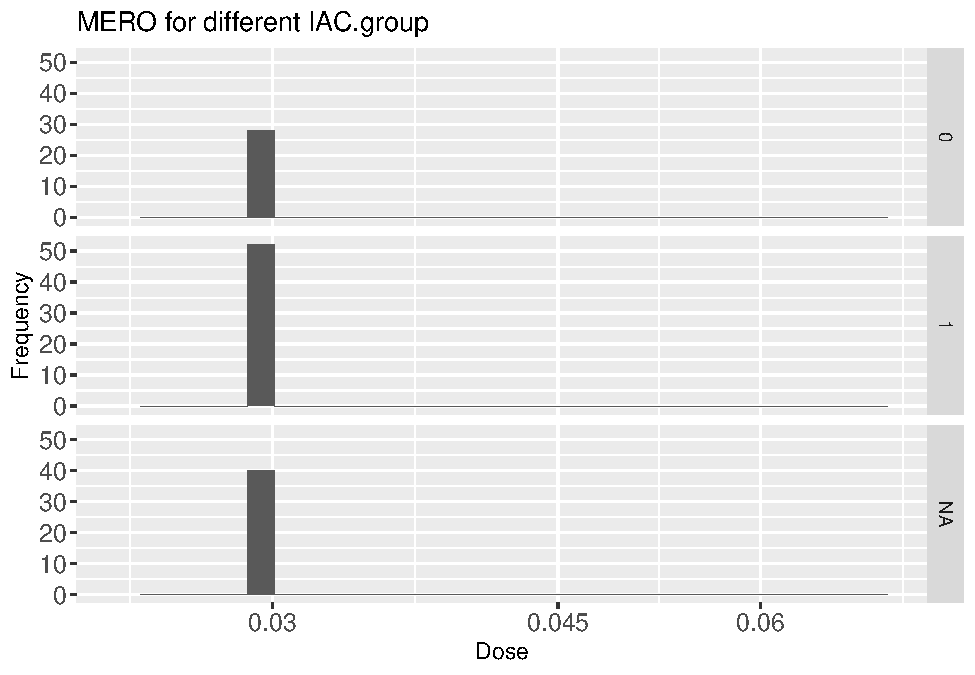
\includegraphics{Verteilungen_files/figure-latex/unnamed-chunk-6-1.pdf}

\begin{Shaded}
\begin{Highlighting}[]
  \KeywordTok{graphisch}\NormalTok{(}\StringTok{"IAC.group"}\NormalTok{, }\StringTok{"CIP"}\NormalTok{ , }\FloatTok{0.015}\NormalTok{,   }\DecValTok{8}\NormalTok{   ,   }\FloatTok{0.015}\NormalTok{,   }\DecValTok{4}\NormalTok{     ) }
\end{Highlighting}
\end{Shaded}

\begin{verbatim}
## [1] "CIP - Resistance, IAC            :"
## [1] "  Median             <= 0.015"
## [1] "  Mean   in  0.321 ... 0.333"
## [1] ""
## [1] "CIP - Resistance, no IAC       :"
## [1] "  Median             <= 0.015"
## [1] "  Mean   in  0.857 ... 0.871"
## [1] ""
\end{verbatim}

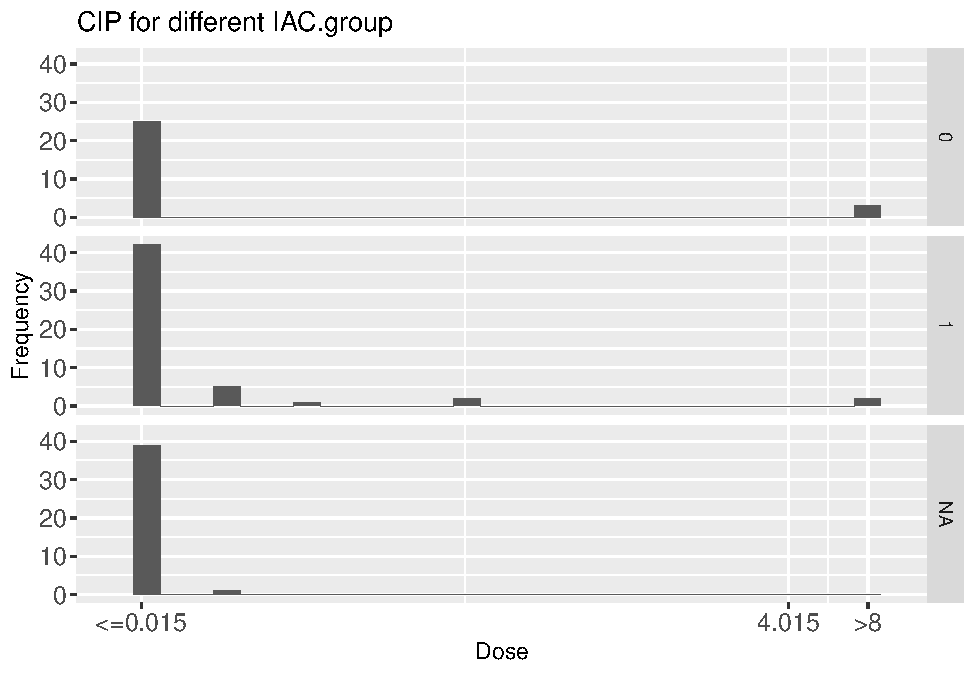
\includegraphics{Verteilungen_files/figure-latex/unnamed-chunk-7-1.pdf}

\begin{Shaded}
\begin{Highlighting}[]
   \KeywordTok{graphisch}\NormalTok{(}\StringTok{"IAC.group"}\NormalTok{,}\StringTok{"AZI"}\NormalTok{ , }\DecValTok{2}\NormalTok{,}\DecValTok{64}\NormalTok{,   }\DecValTok{1}\NormalTok{,}\DecValTok{10}\NormalTok{)}
\end{Highlighting}
\end{Shaded}

\begin{verbatim}
## [1] "AZI - Resistance, IAC            :"
## [1] "  Median             = 8"
## [1] "  Mean   in  6.538 ... 6.615"
## [1] ""
## [1] "AZI - Resistance, no IAC       :"
## [1] "  Median             = 8"
## [1] "  Mean   in  7.286 ... 7.357"
## [1] ""
\end{verbatim}

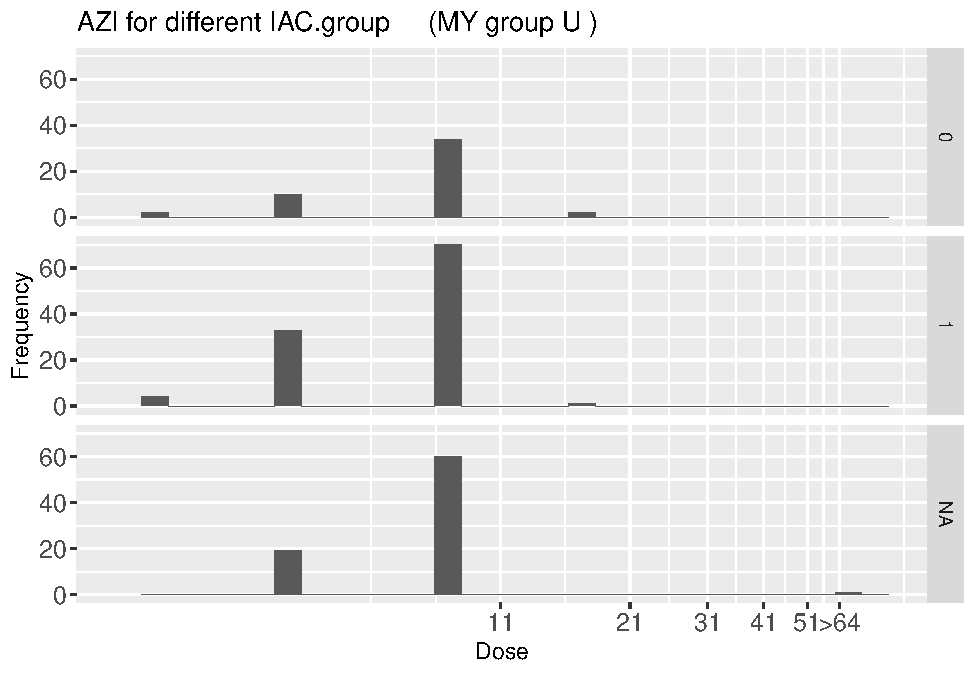
\includegraphics{Verteilungen_files/figure-latex/unnamed-chunk-8-1.pdf}

\begin{Shaded}
\begin{Highlighting}[]
   \KeywordTok{graphisch}\NormalTok{(}\StringTok{"IAC.group"}\NormalTok{, }\StringTok{"GEN"}\NormalTok{ , }\FloatTok{0.5}\NormalTok{  ,  }\DecValTok{16}\NormalTok{   ,   }\FloatTok{0.5}\NormalTok{  ,   }\DecValTok{4}\NormalTok{    )}
\end{Highlighting}
\end{Shaded}

\begin{verbatim}
## [1] "GEN - Resistance, IAC            :"
## [1] "  Median             <= 0.5"
## [1] "  Mean   in  1.827 ... 2.192"
## [1] ""
## [1] "GEN - Resistance, no IAC       :"
## [1] "  Median             <= 0.5"
## [1] "  Mean   in  0.679 ... 1.107"
## [1] ""
\end{verbatim}

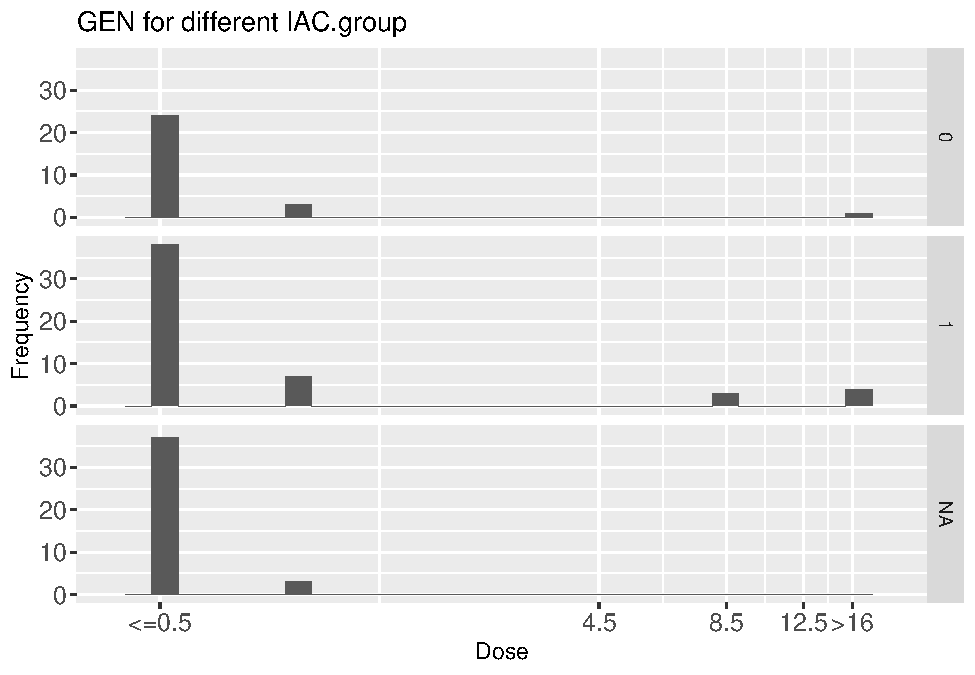
\includegraphics{Verteilungen_files/figure-latex/unnamed-chunk-9-1.pdf}

\begin{Shaded}
\begin{Highlighting}[]
   \KeywordTok{graphisch}\NormalTok{(}\StringTok{"IAC.group"}\NormalTok{, }\StringTok{"TGC"}\NormalTok{ , }\FloatTok{0.25}\NormalTok{ ,  }\FloatTok{-0.5}\NormalTok{ ,   }\FloatTok{0.25}\NormalTok{ ,   }\FloatTok{0.25}\NormalTok{ )  }
\end{Highlighting}
\end{Shaded}

\begin{verbatim}
## [1] "TGC - Resistance, IAC            :"
## [1] "  Median             <= 0.25"
## [1] "  Mean   in  0.058 ... 0.279"
## [1] ""
## [1] "TGC - Resistance, no IAC       :"
## [1] "  Median             <= 0.25"
## [1] "  Mean   in  0.071 ... 0.286"
## [1] ""
\end{verbatim}

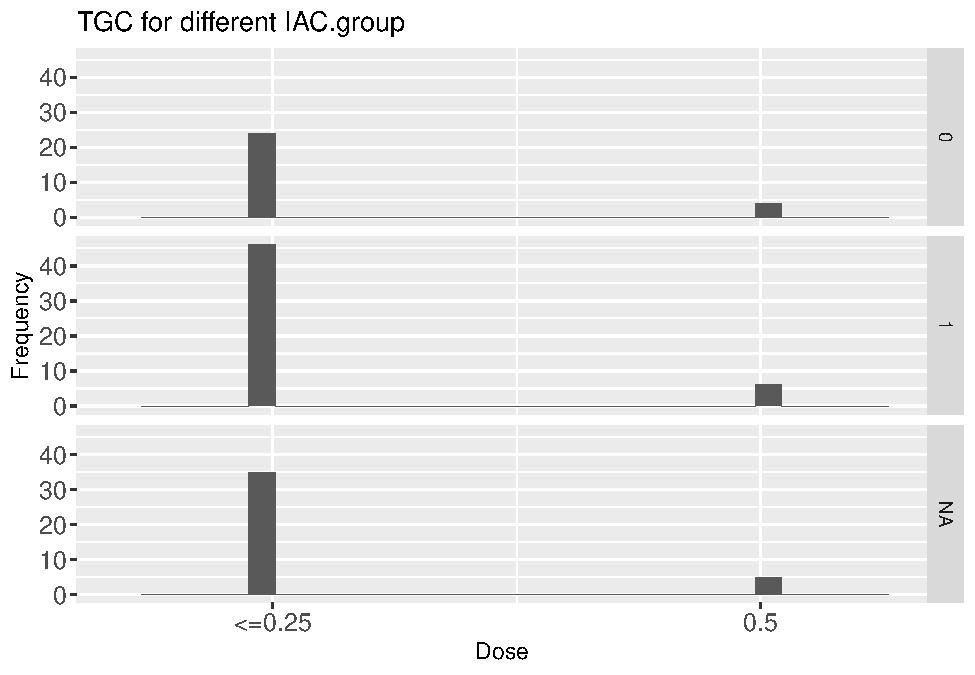
\includegraphics{Verteilungen_files/figure-latex/unnamed-chunk-10-1.pdf}

\begin{Shaded}
\begin{Highlighting}[]
   \KeywordTok{graphisch}\NormalTok{(}\StringTok{"IAC.group"}\NormalTok{, }\StringTok{"TAZ"}\NormalTok{ , }\FloatTok{0.25}\NormalTok{,}\OperatorTok{-}\DecValTok{1}\NormalTok{,   }\FloatTok{0.25}\NormalTok{,}\FloatTok{0.25}\NormalTok{ )  }
\end{Highlighting}
\end{Shaded}

\begin{verbatim}
## [1] "TAZ - Resistance, IAC            :"
## [1] "  Median             <= 0.25"
## [1] "  Mean   in  0.000 ... 0.250"
## [1] ""
## [1] "TAZ - Resistance, no IAC       :"
## [1] "  Median             <= 0.25"
## [1] "  Mean   in  0.125 ... 0.339"
## [1] ""
\end{verbatim}

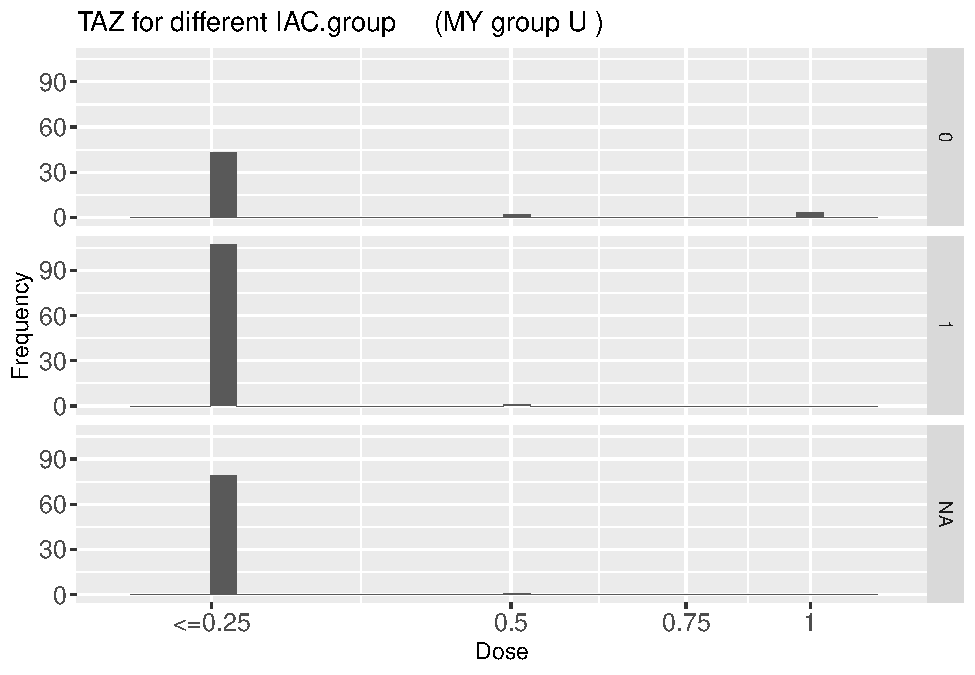
\includegraphics{Verteilungen_files/figure-latex/unnamed-chunk-11-1.pdf}

\begin{Shaded}
\begin{Highlighting}[]
  \KeywordTok{graphisch}\NormalTok{(}\StringTok{"IAC.group"}\NormalTok{, }\StringTok{"FOT"}\NormalTok{ , }\FloatTok{0.25}\NormalTok{,}\DecValTok{4}\NormalTok{   ,   }\FloatTok{0.25}\NormalTok{,}\DecValTok{1}\NormalTok{     )  }
\end{Highlighting}
\end{Shaded}

\begin{verbatim}
## [1] "FOT - Resistance, IAC            :"
## [1] "  Median             <= 0.25"
## [1] "  Mean   in  0.000 ... 0.250"
## [1] ""
## [1] "FOT - Resistance, no IAC       :"
## [1] "  Median             <= 0.25"
## [1] "  Mean   in  0.429 ... 0.652"
## [1] ""
\end{verbatim}

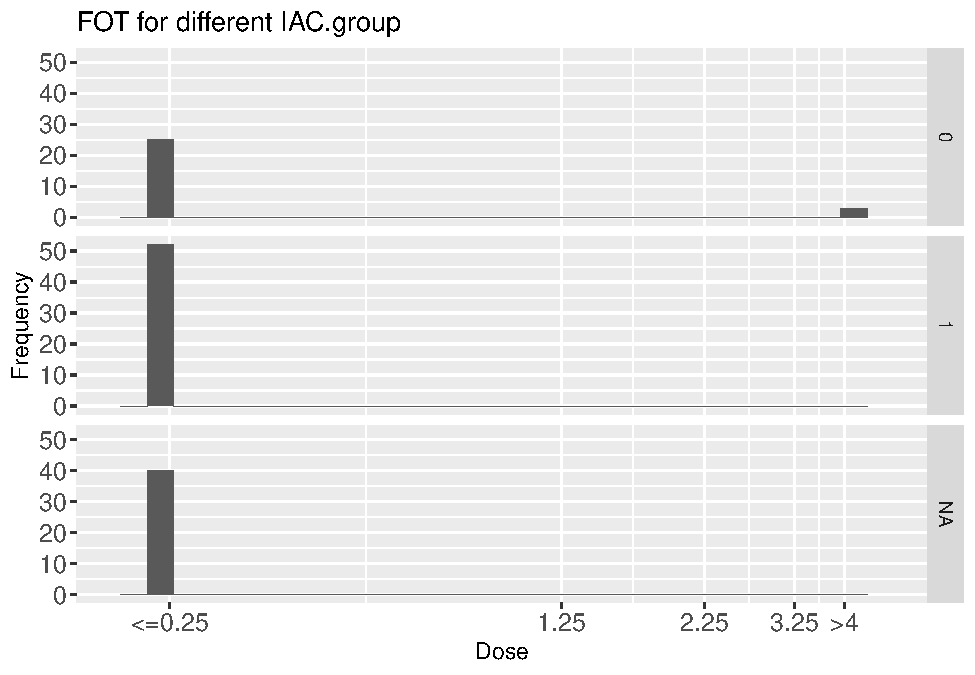
\includegraphics{Verteilungen_files/figure-latex/unnamed-chunk-12-1.pdf}

\begin{Shaded}
\begin{Highlighting}[]
   \KeywordTok{graphisch}\NormalTok{(}\StringTok{"IAC.group"}\NormalTok{, }\StringTok{"CHL"}\NormalTok{ , }\DecValTok{8}\NormalTok{    ,  }\DecValTok{64}\NormalTok{   ,   }\DecValTok{8}\NormalTok{,}\DecValTok{16}\NormalTok{   ) }
\end{Highlighting}
\end{Shaded}

\begin{verbatim}
## [1] "CHL - Resistance, IAC            :"
## [1] "  Median             <= 8"
## [1] "  Mean   in  12.615 ... 18.923"
## [1] ""
## [1] "CHL - Resistance, no IAC       :"
## [1] "  Median             <= 8"
## [1] "  Mean   in  12.571 ... 18.571"
## [1] ""
\end{verbatim}

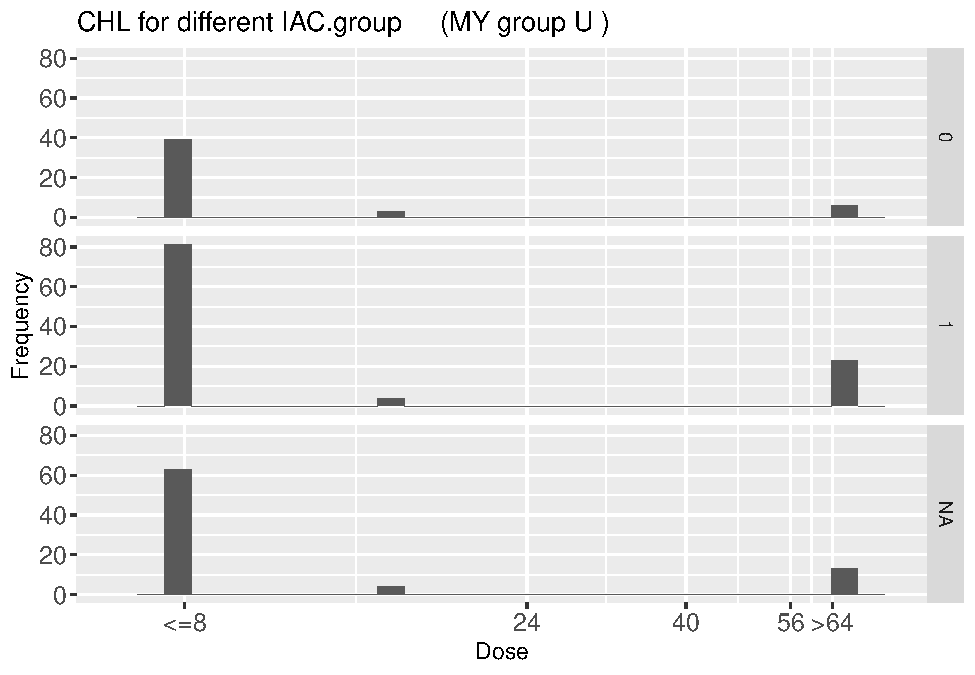
\includegraphics{Verteilungen_files/figure-latex/unnamed-chunk-13-1.pdf}

\begin{Shaded}
\begin{Highlighting}[]
   \KeywordTok{graphisch}\NormalTok{(}\StringTok{"IAC.group"}\NormalTok{, }\StringTok{"NAL"}\NormalTok{ , }\DecValTok{4}\NormalTok{,}\DecValTok{64}\NormalTok{,   }\DecValTok{4}\NormalTok{,}\DecValTok{16}\NormalTok{    ) }
\end{Highlighting}
\end{Shaded}

\begin{verbatim}
## [1] "NAL - Resistance, IAC            :"
## [1] "  Median             <= 4"
## [1] "  Mean   in  4.000 ... 7.615"
## [1] ""
## [1] "NAL - Resistance, no IAC       :"
## [1] "  Median             <= 4"
## [1] "  Mean   in  6.857 ... 10.429"
## [1] ""
\end{verbatim}

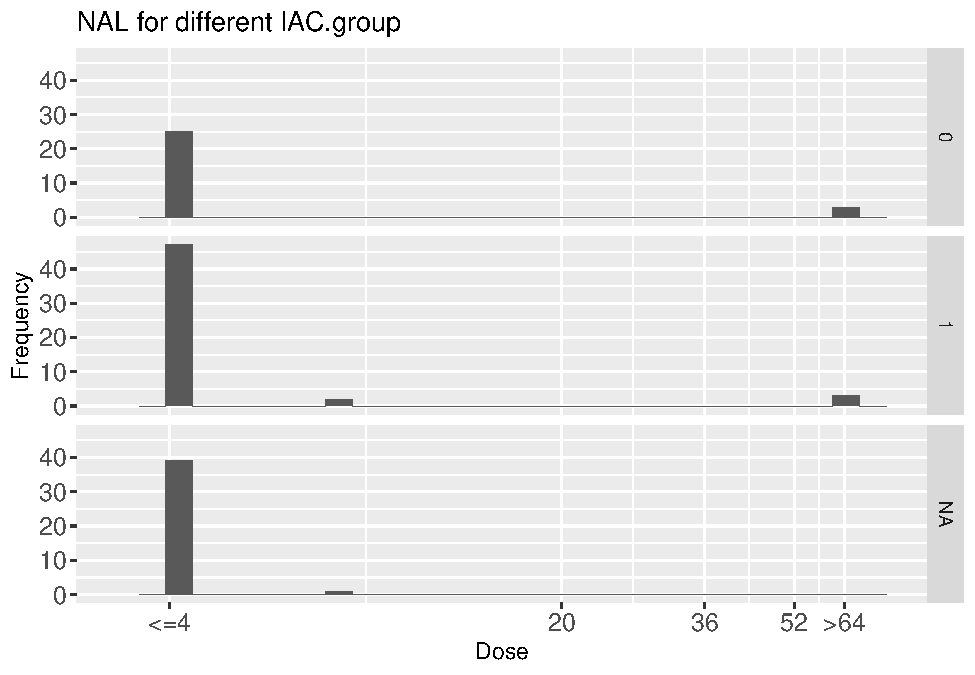
\includegraphics{Verteilungen_files/figure-latex/unnamed-chunk-14-1.pdf}

\begin{Shaded}
\begin{Highlighting}[]
   \KeywordTok{graphisch}\NormalTok{(}\StringTok{"IAC.group"}\NormalTok{, }\StringTok{"TET"}\NormalTok{ , }\DecValTok{2}\NormalTok{,}\DecValTok{32}\NormalTok{,   }\DecValTok{2}\NormalTok{,}\DecValTok{8}\NormalTok{    ) }
\end{Highlighting}
\end{Shaded}

\begin{verbatim}
## [1] "TET - Resistance, IAC            :"
## [1] "  Median             = 4"
## [1] "  Mean   in  12.385 ... 13.346"
## [1] ""
## [1] "TET - Resistance, no IAC       :"
## [1] "  Median             <= 2"
## [1] "  Mean   in  11.714 ... 12.857"
## [1] ""
\end{verbatim}

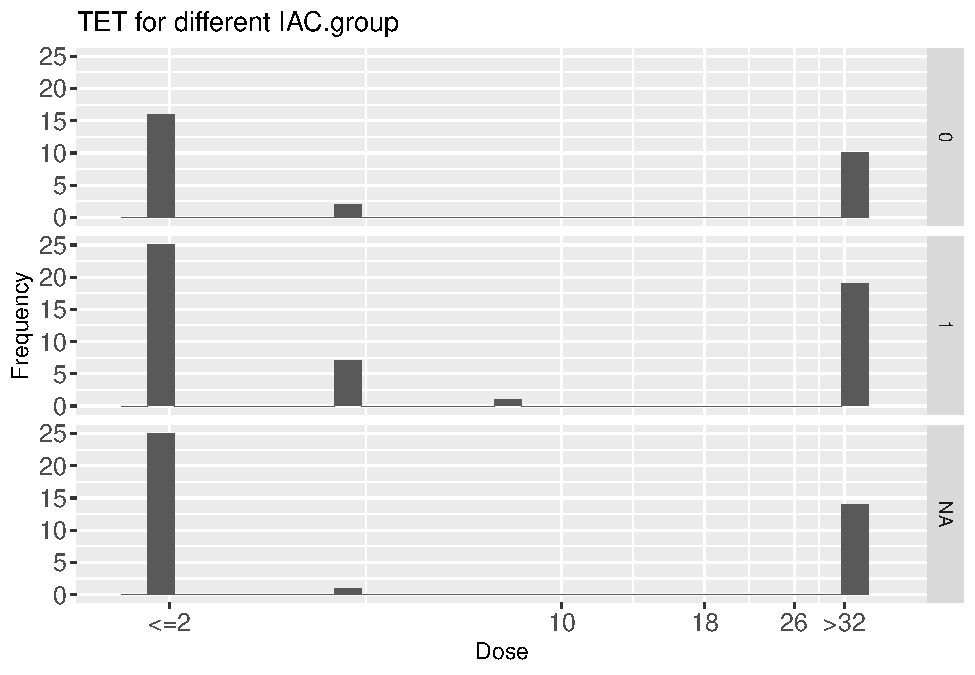
\includegraphics{Verteilungen_files/figure-latex/unnamed-chunk-15-1.pdf}

\begin{Shaded}
\begin{Highlighting}[]
   \KeywordTok{graphisch}\NormalTok{(}\StringTok{"IAC.group"}\NormalTok{, }\StringTok{"TMP"}\NormalTok{ , }\FloatTok{0.25}\NormalTok{ ,  }\DecValTok{16}\NormalTok{   ,   }\FloatTok{0.25}\NormalTok{,}\DecValTok{8}\NormalTok{    ) }
\end{Highlighting}
\end{Shaded}

\begin{verbatim}
## [1] "TMP - Resistance, IAC            :"
## [1] "  Median             = 0.5"
## [1] "  Mean   in  4.048 ... 4.077"
## [1] ""
## [1] "TMP - Resistance, no IAC       :"
## [1] "  Median             = 0.5"
## [1] "  Mean   in  5.375 ... 5.429"
## [1] ""
\end{verbatim}

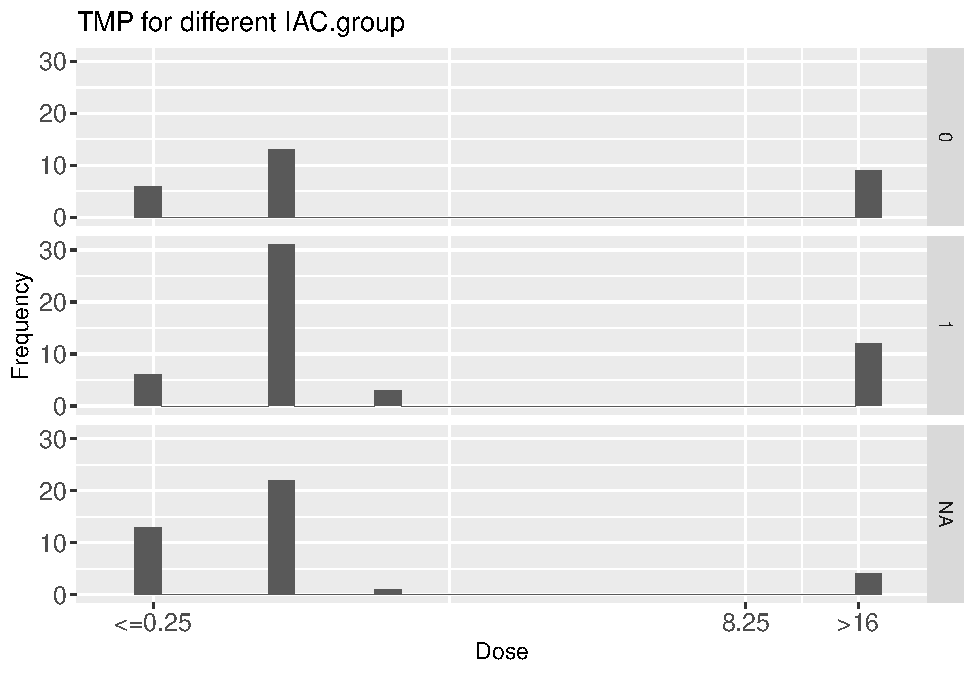
\includegraphics{Verteilungen_files/figure-latex/unnamed-chunk-16-1.pdf}

\begin{Shaded}
\begin{Highlighting}[]
   \KeywordTok{graphisch}\NormalTok{(}\StringTok{"IAC.group"}\NormalTok{, }\StringTok{"SMX"}\NormalTok{ , }\DecValTok{8}\NormalTok{    , }\DecValTok{512}\NormalTok{   ,   }\DecValTok{8}\NormalTok{,}\DecValTok{256}\NormalTok{    ) }
\end{Highlighting}
\end{Shaded}

\begin{verbatim}
## [1] "SMX - Resistance, IAC            :"
## [1] "  Median             = 16"
## [1] "  Mean   in  196.000 ... 197.385"
## [1] ""
## [1] "SMX - Resistance, no IAC       :"
## [1] "  Median             = 16"
## [1] "  Mean   in  225.143 ... 227.143"
## [1] ""
\end{verbatim}

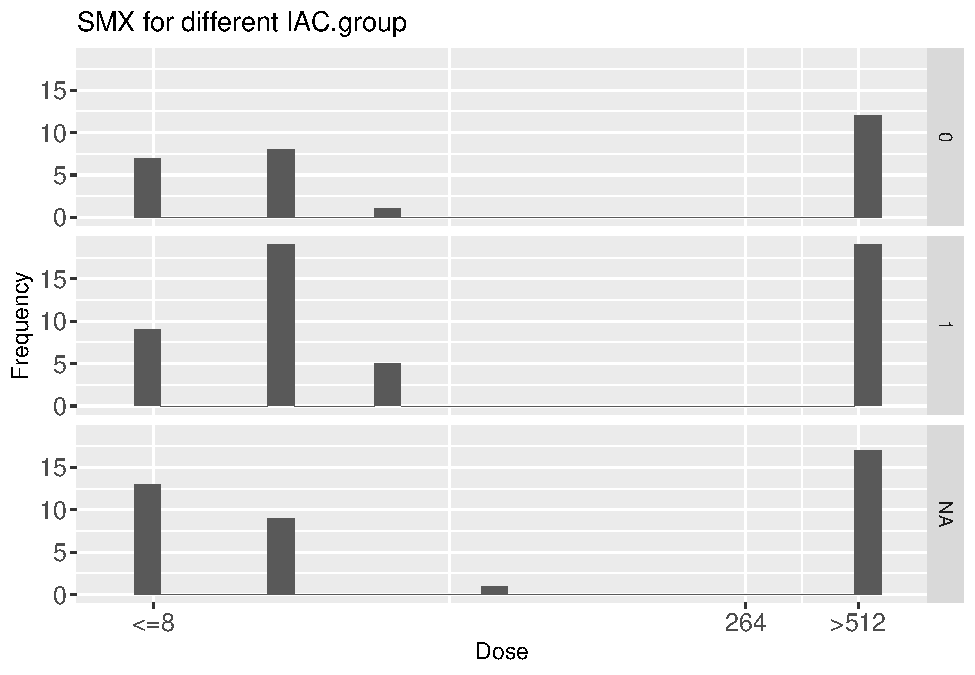
\includegraphics{Verteilungen_files/figure-latex/unnamed-chunk-17-1.pdf}

\begin{Shaded}
\begin{Highlighting}[]
   \CommentTok{#stop the script - by error }
\end{Highlighting}
\end{Shaded}

Die Mittelwerte der Resistenz sind für 5 Antibiotika vergleichbar (AMP,
MERO, TGC, TAZ, CHL), für GEN tendenziell grösser im Fall \emph{Ill
Animals in Calving box}, für 3 Antibiotika tendenziell kleiner in diesem
Fall (ZIP, AZI, NAL), für TET definitv grösser in diesem Fall und für 3
Antibiotika definitiv kleiner in diesem Fall (FOT, TMP, SMX). Diese
Relationen sind im wesentlichen gleich gerichtet wie in WM - keine WM.

Der Vergleich des Medians der 2 Gruppen zeigt Unterschiede nur für TET
und SMX, in der gleichen Richtung wie der Mittelwert. Deshalb diskutiere
ich den Median nicht weiter.

\hypertarget{other-live-stock---gruppen}{%
\subsection{Other Live Stock -
Gruppen}\label{other-live-stock---gruppen}}

Mit ``OLS'' abgekürzt.

\begin{Shaded}
\begin{Highlighting}[]
  \KeywordTok{graphisch}\NormalTok{(}\StringTok{"OLS.group"}\NormalTok{, }\StringTok{"AMP"}\NormalTok{, }\DecValTok{1}\NormalTok{,}\DecValTok{32}\NormalTok{, }\DecValTok{1}\NormalTok{,}\DecValTok{8}\NormalTok{)}
\end{Highlighting}
\end{Shaded}

\begin{verbatim}
## [1] "AMP - Resistance, OLS            :"
## [1] "  Median             = 4"
## [1] "  Mean   =  15.077"
## [1] ""
## [1] "AMP - Resistance, no OLS       :"
## [1] "  Median             = 4"
## [1] "  Mean   =  10.471"
## [1] ""
\end{verbatim}

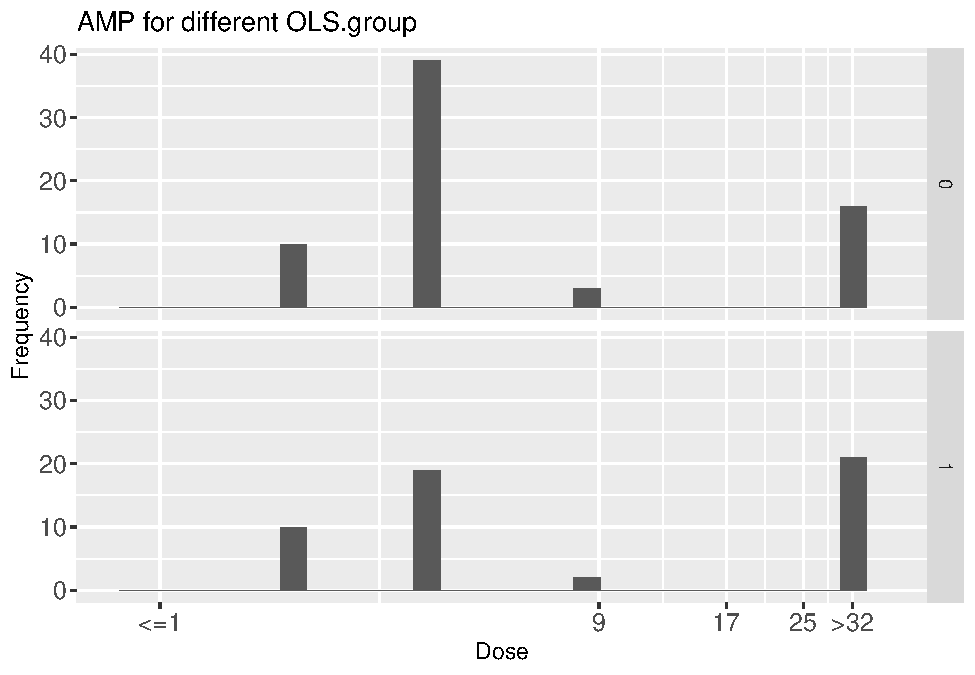
\includegraphics{Verteilungen_files/figure-latex/unnamed-chunk-18-1.pdf}

\begin{Shaded}
\begin{Highlighting}[]
  \KeywordTok{graphisch}\NormalTok{(}\StringTok{"OLS.group"}\NormalTok{, }\StringTok{"MERO"}\NormalTok{, }\FloatTok{0.03}\NormalTok{ ,  }\FloatTok{-0.06}\NormalTok{,   }\FloatTok{0.015}\NormalTok{,   }\FloatTok{0.015}\NormalTok{ )}
\end{Highlighting}
\end{Shaded}

\begin{verbatim}
## [1] "MERO - Resistance, OLS            :"
## [1] "  Median             <= 0.03"
## [1] "  Mean   in  0.000 ... 0.030"
## [1] ""
## [1] "MERO - Resistance, no OLS       :"
## [1] "  Median             <= 0.03"
## [1] "  Mean   in  0.000 ... 0.030"
## [1] ""
\end{verbatim}

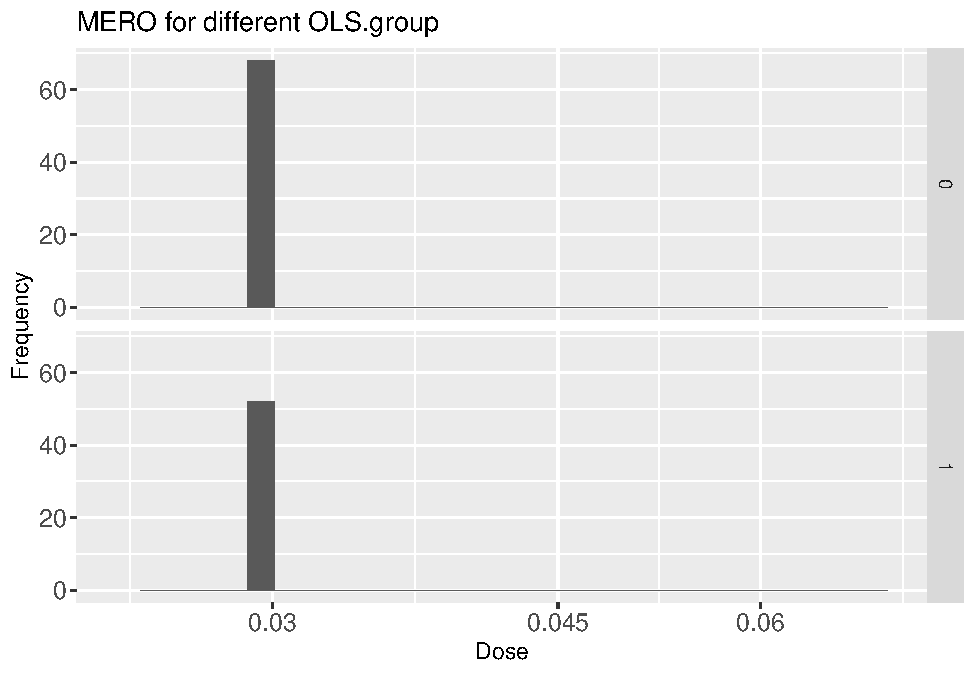
\includegraphics{Verteilungen_files/figure-latex/unnamed-chunk-19-1.pdf}

\begin{Shaded}
\begin{Highlighting}[]
  \KeywordTok{graphisch}\NormalTok{(}\StringTok{"OLS.group"}\NormalTok{, }\StringTok{"CIP"}\NormalTok{ , }\FloatTok{0.015}\NormalTok{,   }\DecValTok{8}\NormalTok{   ,   }\FloatTok{0.015}\NormalTok{,   }\DecValTok{4}\NormalTok{     ) }
\end{Highlighting}
\end{Shaded}

\begin{verbatim}
## [1] "CIP - Resistance, OLS            :"
## [1] "  Median             <= 0.015"
## [1] "  Mean   in  0.467 ... 0.480"
## [1] ""
## [1] "CIP - Resistance, no OLS       :"
## [1] "  Median             <= 0.015"
## [1] "  Mean   in  0.242 ... 0.255"
## [1] ""
\end{verbatim}

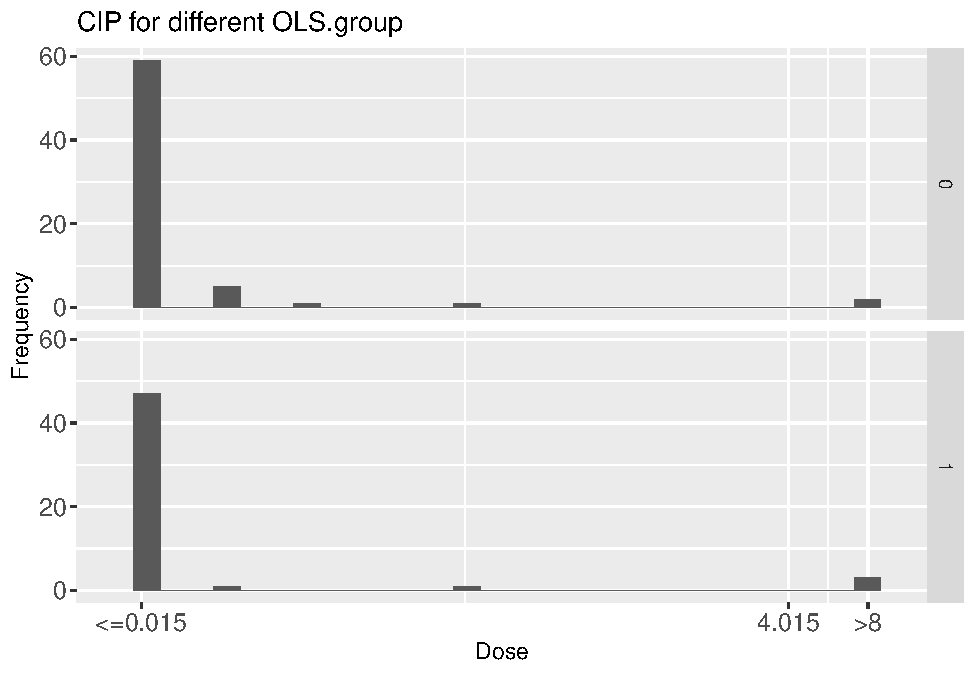
\includegraphics{Verteilungen_files/figure-latex/unnamed-chunk-20-1.pdf}

\begin{Shaded}
\begin{Highlighting}[]
  \KeywordTok{graphisch}\NormalTok{(}\StringTok{"OLS.group"}\NormalTok{,}\StringTok{"AZI"}\NormalTok{, }\DecValTok{2}\NormalTok{,}\DecValTok{64}\NormalTok{, }\DecValTok{1}\NormalTok{,}\DecValTok{10}\NormalTok{    )}
\end{Highlighting}
\end{Shaded}

\begin{verbatim}
## [1] "AZI - Resistance, OLS            :"
## [1] "  Median             = 8"
## [1] "  Mean   in  7.615 ... 7.692"
## [1] ""
## [1] "AZI - Resistance, no OLS       :"
## [1] "  Median             = 8"
## [1] "  Mean   in  6.882 ... 6.912"
## [1] ""
\end{verbatim}

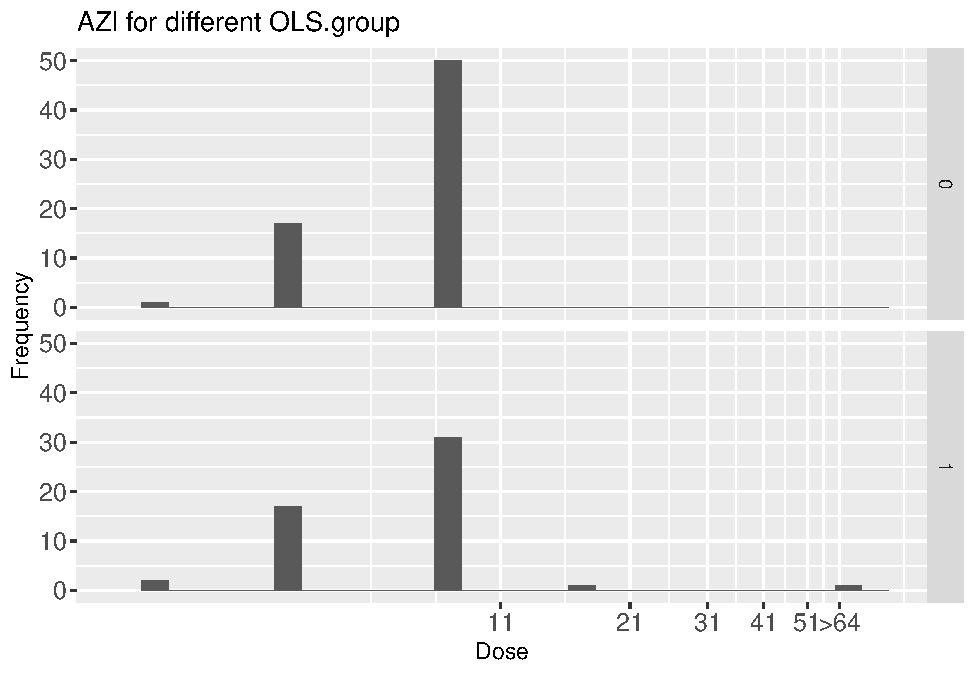
\includegraphics{Verteilungen_files/figure-latex/unnamed-chunk-21-1.pdf}

\begin{Shaded}
\begin{Highlighting}[]
  \KeywordTok{graphisch}\NormalTok{(}\StringTok{"OLS.group"}\NormalTok{, }\StringTok{"GEN"}\NormalTok{ , }\FloatTok{0.5}\NormalTok{  ,  }\DecValTok{16}\NormalTok{   ,   }\FloatTok{0.5}\NormalTok{  ,   }\DecValTok{4}\NormalTok{    )}
\end{Highlighting}
\end{Shaded}

\begin{verbatim}
## [1] "GEN - Resistance, OLS            :"
## [1] "  Median             <= 0.5"
## [1] "  Mean   in  1.173 ... 1.577"
## [1] ""
## [1] "GEN - Resistance, no OLS       :"
## [1] "  Median             <= 0.5"
## [1] "  Mean   in  0.824 ... 1.243"
## [1] ""
\end{verbatim}

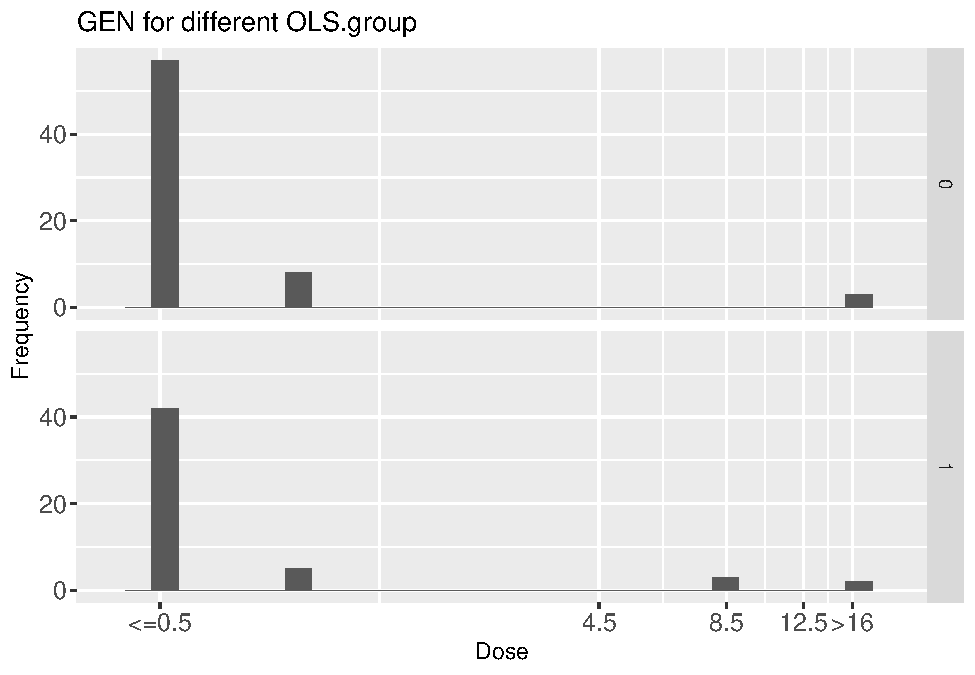
\includegraphics{Verteilungen_files/figure-latex/unnamed-chunk-22-1.pdf}

\begin{Shaded}
\begin{Highlighting}[]
  \KeywordTok{graphisch}\NormalTok{(}\StringTok{"OLS.group"}\NormalTok{, }\StringTok{"TGC"}\NormalTok{ , }\FloatTok{0.25}\NormalTok{ ,  }\FloatTok{-0.5}\NormalTok{ ,   }\FloatTok{0.25}\NormalTok{ ,   }\FloatTok{0.25}\NormalTok{ )  }
\end{Highlighting}
\end{Shaded}

\begin{verbatim}
## [1] "TGC - Resistance, OLS            :"
## [1] "  Median             <= 0.25"
## [1] "  Mean   in  0.029 ... 0.264"
## [1] ""
## [1] "TGC - Resistance, no OLS       :"
## [1] "  Median             <= 0.25"
## [1] "  Mean   in  0.088 ... 0.294"
## [1] ""
\end{verbatim}

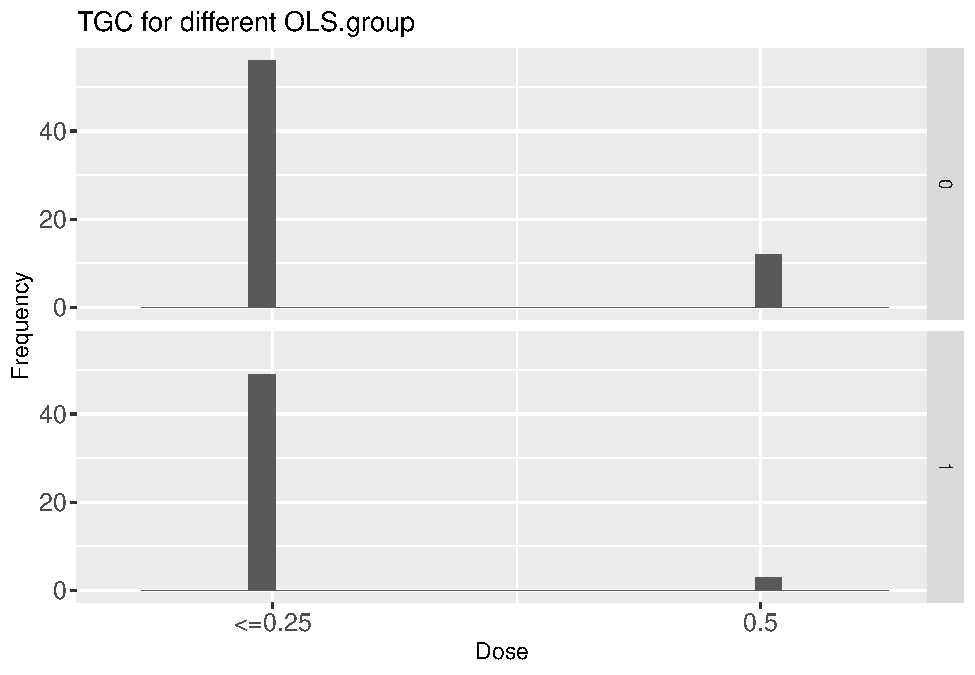
\includegraphics{Verteilungen_files/figure-latex/unnamed-chunk-23-1.pdf}

\begin{Shaded}
\begin{Highlighting}[]
  \KeywordTok{graphisch}\NormalTok{(}\StringTok{"OLS.group"}\NormalTok{, }\StringTok{"TAZ"}\NormalTok{ , }\FloatTok{0.25}\NormalTok{,}\OperatorTok{-}\DecValTok{1}\NormalTok{   ,   }\FloatTok{0.25}\NormalTok{,}\FloatTok{0.25}\NormalTok{ )  }
\end{Highlighting}
\end{Shaded}

\begin{verbatim}
## [1] "TAZ - Resistance, OLS            :"
## [1] "  Median             <= 0.25"
## [1] "  Mean   in  0.067 ... 0.298"
## [1] ""
## [1] "TAZ - Resistance, no OLS       :"
## [1] "  Median             <= 0.25"
## [1] "  Mean   in  0.000 ... 0.250"
## [1] ""
\end{verbatim}

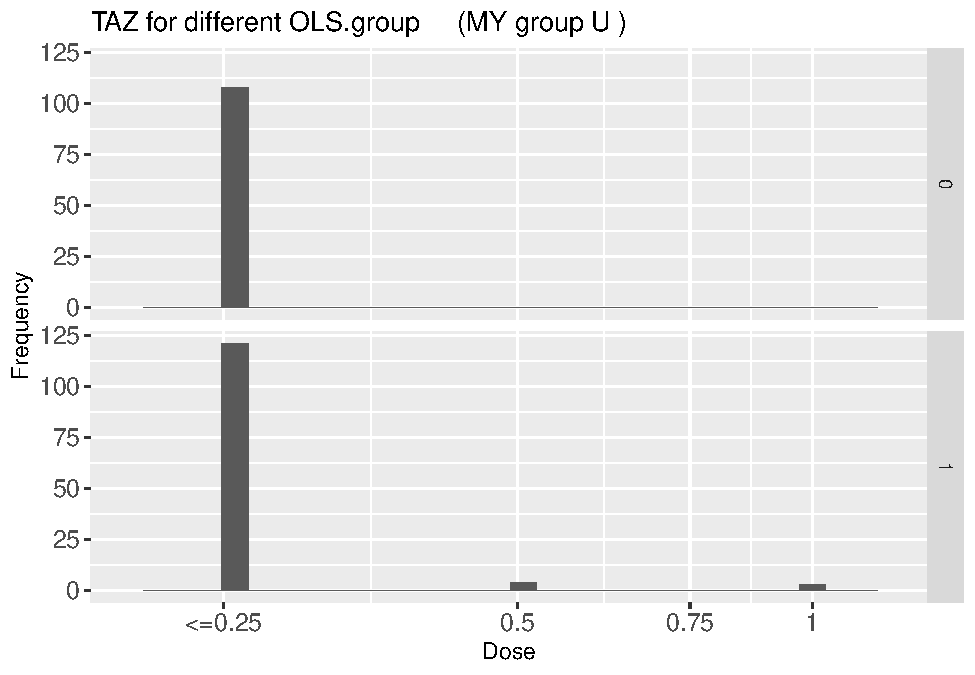
\includegraphics{Verteilungen_files/figure-latex/unnamed-chunk-24-1.pdf}

\begin{Shaded}
\begin{Highlighting}[]
  \KeywordTok{graphisch}\NormalTok{(}\StringTok{"OLS.group"}\NormalTok{, }\StringTok{"FOT"}\NormalTok{ , }\FloatTok{0.25}\NormalTok{ ,   }\DecValTok{4}\NormalTok{   ,   }\FloatTok{0.25}\NormalTok{ ,   }\DecValTok{1}\NormalTok{     )  }
\end{Highlighting}
\end{Shaded}

\begin{verbatim}
## [1] "FOT - Resistance, OLS            :"
## [1] "  Median             <= 0.25"
## [1] "  Mean   in  0.231 ... 0.466"
## [1] ""
## [1] "FOT - Resistance, no OLS       :"
## [1] "  Median             <= 0.25"
## [1] "  Mean   in  0.000 ... 0.250"
## [1] ""
\end{verbatim}

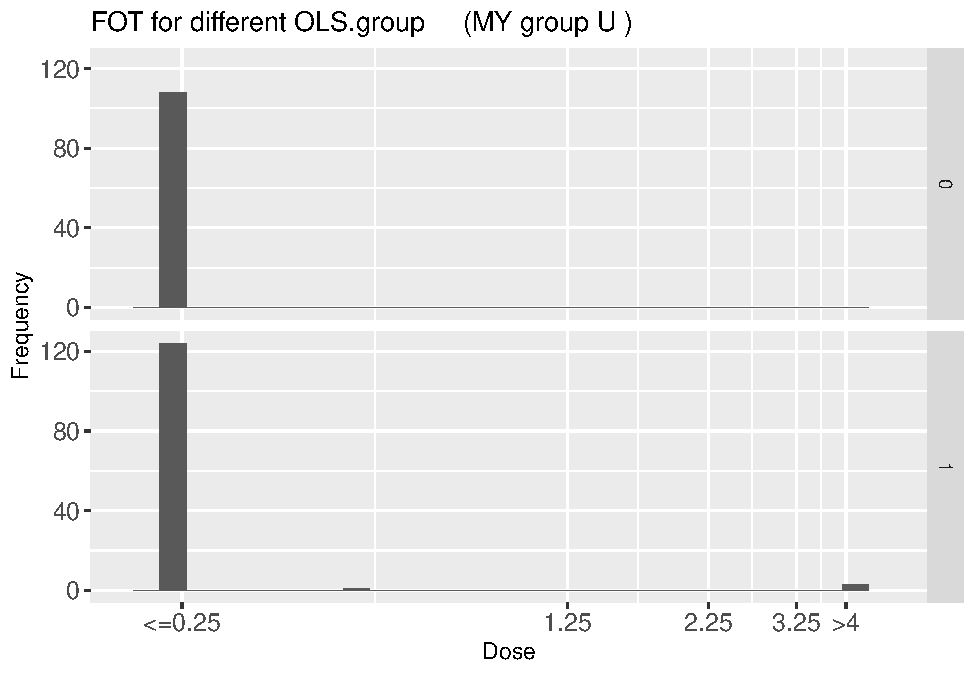
\includegraphics{Verteilungen_files/figure-latex/unnamed-chunk-25-1.pdf}

\begin{Shaded}
\begin{Highlighting}[]
  \KeywordTok{graphisch}\NormalTok{(}\StringTok{"OLS.group"}\NormalTok{, }\StringTok{"CHL"}\NormalTok{ , }\DecValTok{8}\NormalTok{    ,  }\DecValTok{64}\NormalTok{   ,   }\DecValTok{8}\NormalTok{,}\DecValTok{16}\NormalTok{    ) }
\end{Highlighting}
\end{Shaded}

\begin{verbatim}
## [1] "CHL - Resistance, OLS            :"
## [1] "  Median             <= 8"
## [1] "  Mean   in  19.077 ... 24.462"
## [1] ""
## [1] "CHL - Resistance, no OLS       :"
## [1] "  Median             <= 8"
## [1] "  Mean   in  9.176 ... 15.765"
## [1] ""
\end{verbatim}

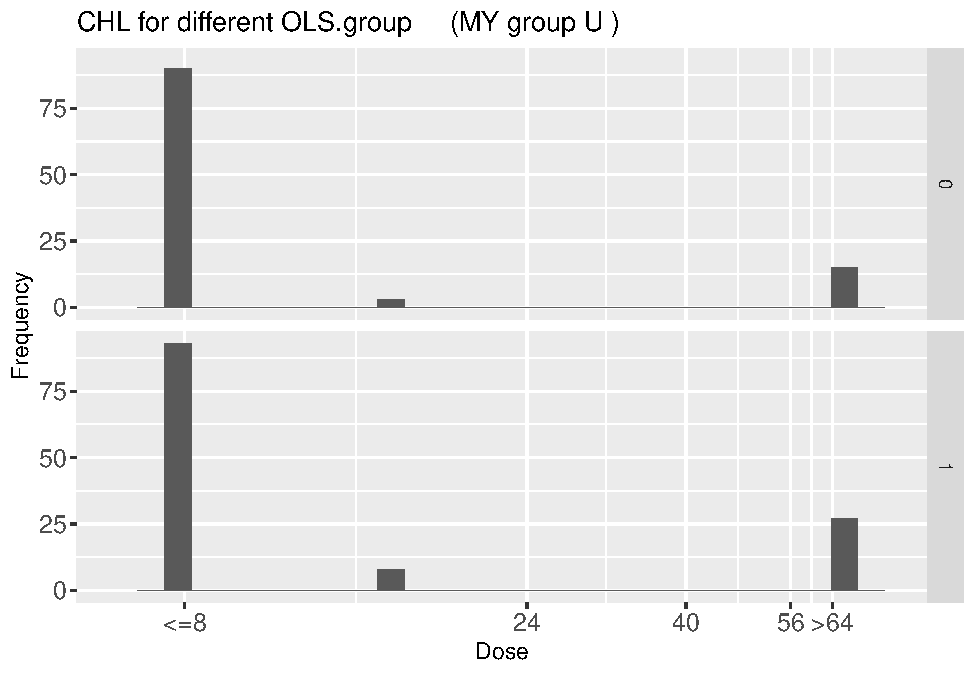
\includegraphics{Verteilungen_files/figure-latex/unnamed-chunk-26-1.pdf}

\begin{Shaded}
\begin{Highlighting}[]
  \KeywordTok{graphisch}\NormalTok{(}\StringTok{"OLS.group"}\NormalTok{, }\StringTok{"NAL"}\NormalTok{ , }\DecValTok{4}\NormalTok{    ,  }\DecValTok{64}\NormalTok{   ,   }\DecValTok{4}\NormalTok{,}\DecValTok{16}\NormalTok{    ) }
\end{Highlighting}
\end{Shaded}

\begin{verbatim}
## [1] "NAL - Resistance, OLS            :"
## [1] "  Median             <= 4"
## [1] "  Mean   in  4.000 ... 7.615"
## [1] ""
## [1] "NAL - Resistance, no OLS       :"
## [1] "  Median             <= 4"
## [1] "  Mean   in  2.941 ... 6.706"
## [1] ""
\end{verbatim}

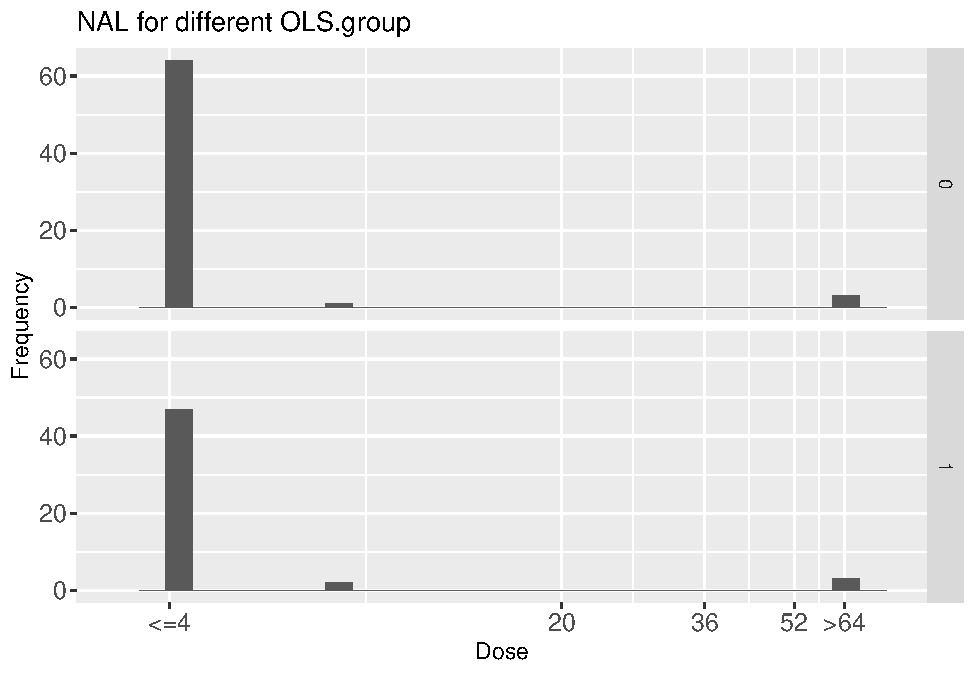
\includegraphics{Verteilungen_files/figure-latex/unnamed-chunk-27-1.pdf}

\begin{Shaded}
\begin{Highlighting}[]
  \KeywordTok{graphisch}\NormalTok{(}\StringTok{"OLS.group"}\NormalTok{, }\StringTok{"TET"}\NormalTok{ , }\DecValTok{2}\NormalTok{    ,  }\DecValTok{32}\NormalTok{   ,   }\DecValTok{2}\NormalTok{,}\DecValTok{8}\NormalTok{    ) }
\end{Highlighting}
\end{Shaded}

\begin{verbatim}
## [1] "TET - Resistance, OLS            :"
## [1] "  Median             = 3"
## [1] "  Mean   in  13.846 ... 14.846"
## [1] ""
## [1] "TET - Resistance, no OLS       :"
## [1] "  Median             <= 2"
## [1] "  Mean   in  10.353 ... 11.529"
## [1] ""
\end{verbatim}

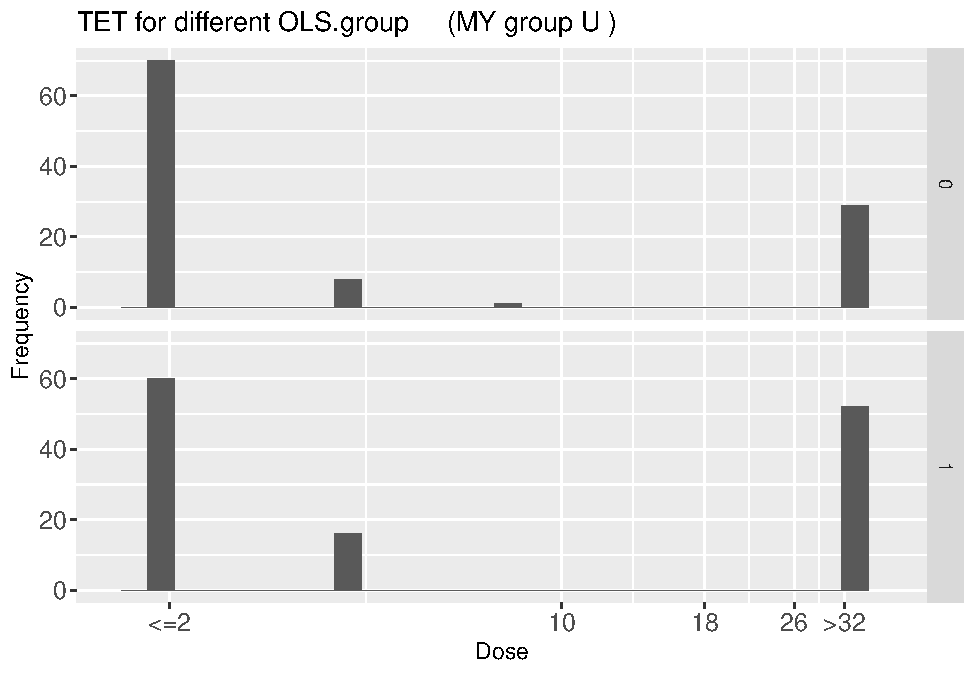
\includegraphics{Verteilungen_files/figure-latex/unnamed-chunk-28-1.pdf}

\begin{Shaded}
\begin{Highlighting}[]
  \KeywordTok{graphisch}\NormalTok{(}\StringTok{"OLS.group"}\NormalTok{, }\StringTok{"TMP"}\NormalTok{ , }\FloatTok{0.25}\NormalTok{ ,  }\DecValTok{16}\NormalTok{   ,   }\FloatTok{0.25}\NormalTok{,}\DecValTok{8}\NormalTok{    ) }
\end{Highlighting}
\end{Shaded}

\begin{verbatim}
## [1] "TMP - Resistance, OLS            :"
## [1] "  Median             = 0.5"
## [1] "  Mean   in  4.817 ... 4.894"
## [1] ""
## [1] "TMP - Resistance, no OLS       :"
## [1] "  Median             = 0.5"
## [1] "  Mean   in  2.743 ... 2.776"
## [1] ""
\end{verbatim}

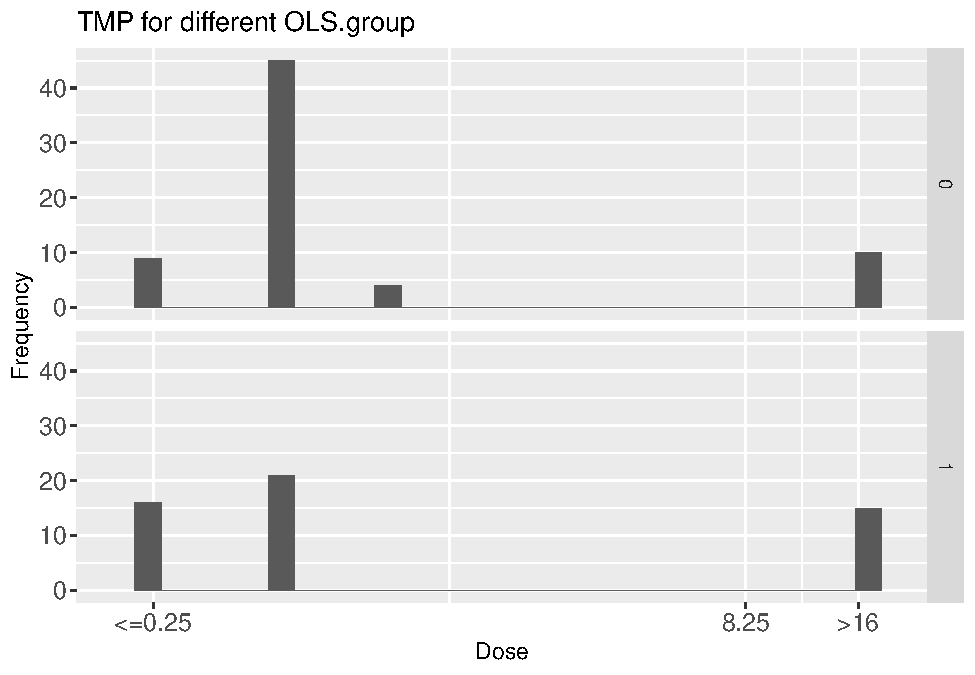
\includegraphics{Verteilungen_files/figure-latex/unnamed-chunk-29-1.pdf}

\begin{Shaded}
\begin{Highlighting}[]
  \KeywordTok{graphisch}\NormalTok{(}\StringTok{"OLS.group"}\NormalTok{, }\StringTok{"SMX"}\NormalTok{ , }\DecValTok{8}\NormalTok{    , }\DecValTok{512}\NormalTok{   ,   }\DecValTok{8}\NormalTok{,}\DecValTok{256}\NormalTok{   ) }
\end{Highlighting}
\end{Shaded}

\begin{verbatim}
## [1] "SMX - Resistance, OLS            :"
## [1] "  Median             = 264"
## [1] "  Mean   in  260.000 ... 262.000"
## [1] ""
## [1] "SMX - Resistance, no OLS       :"
## [1] "  Median             = 16"
## [1] "  Mean   in  174.824 ... 176.706"
## [1] ""
\end{verbatim}

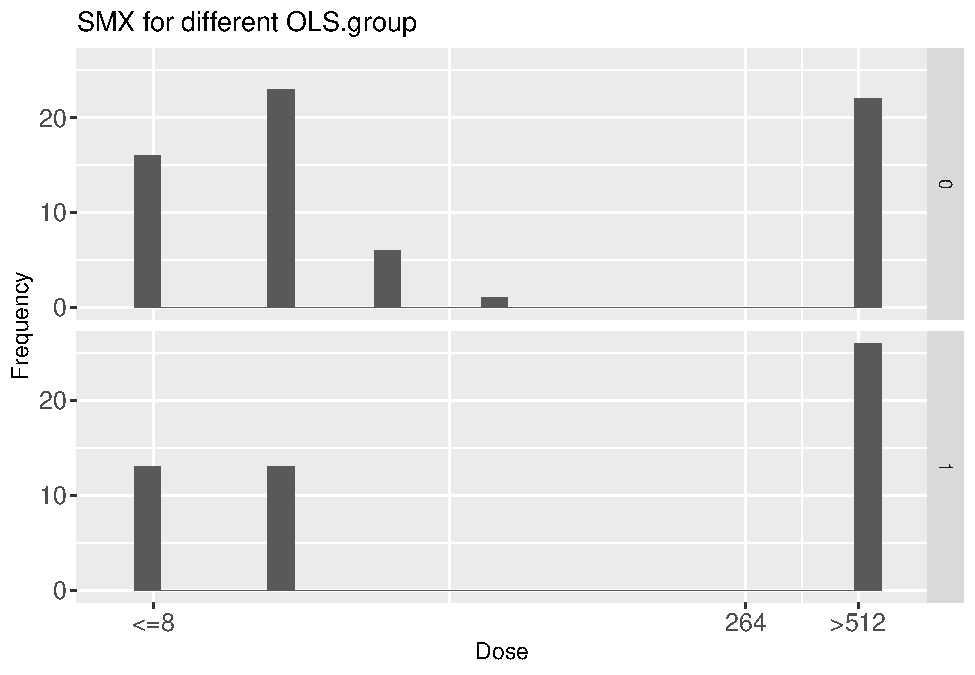
\includegraphics{Verteilungen_files/figure-latex/unnamed-chunk-30-1.pdf}

\begin{Shaded}
\begin{Highlighting}[]
  \CommentTok{#stop the script}
\end{Highlighting}
\end{Shaded}

Die Mittelwerte der Resistenz sind für MERO, GEN und TAZ vergleichbar,
für 5 Antibiotika tendenziell grösser im Fall \emph{Other Livestock}
(CIP, FOT, CHL, NAL, SMX), für TGC tendenziell kleiner in diesem Fall
und für 4 Antibiotika definitiv kleiner in diesem Fall (AMP, AZI, TET,
TMP). Diese Relationen sind im wesentlichen entgegengesetzt zu WM -
keine WM!

\hypertarget{waste-milk---gruppen}{%
\section{Waste Milk - Gruppen}\label{waste-milk---gruppen}}

\begin{Shaded}
\begin{Highlighting}[]
  \KeywordTok{graphisch}\NormalTok{(}\StringTok{"WM.group"}\NormalTok{, }\StringTok{"AMP"}\NormalTok{, }\DecValTok{1}\NormalTok{,}\DecValTok{32}\NormalTok{, }\DecValTok{1}\NormalTok{,}\DecValTok{8}\NormalTok{)}
\end{Highlighting}
\end{Shaded}

\begin{verbatim}
## [1] "AMP - Resistance, WM            :"
## [1] "  Median             = 4"
## [1] "  Mean   =  10.125"
## [1] ""
## [1] "AMP - Resistance, no WM      :"
## [1] "  Median             = 4"
## [1] "  Mean   =  15.143"
## [1] ""
\end{verbatim}

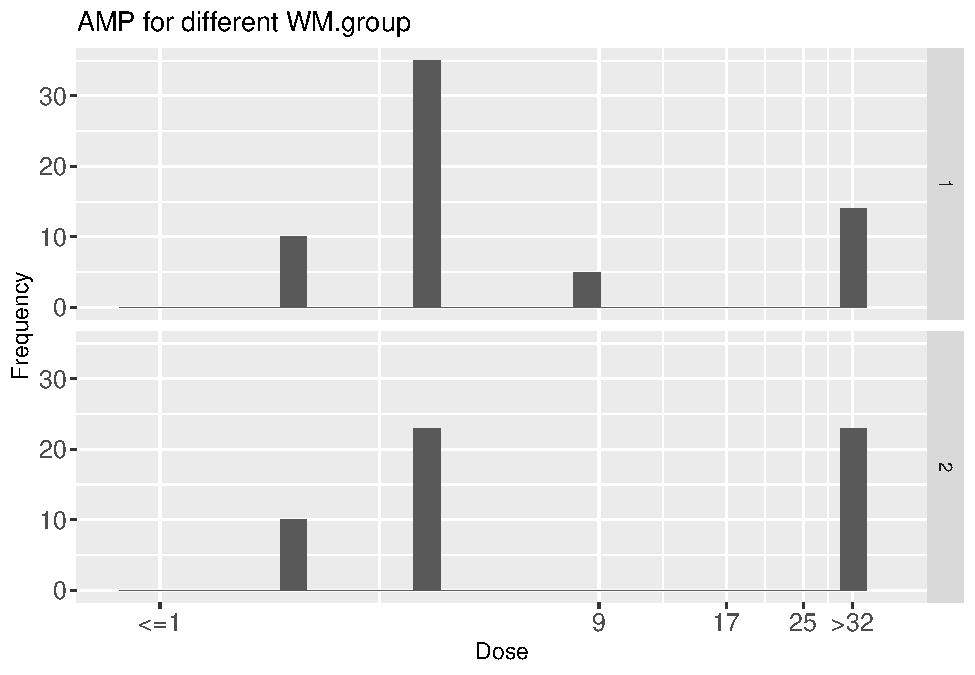
\includegraphics{Verteilungen_files/figure-latex/unnamed-chunk-31-1.pdf}

Der Mittelwert ist höher ohne WM.

\begin{Shaded}
\begin{Highlighting}[]
  \KeywordTok{graphisch}\NormalTok{(}\StringTok{"WM.group"}\NormalTok{, }\StringTok{"MERO"}\NormalTok{, }\FloatTok{.03}\NormalTok{,}\OperatorTok{-}\FloatTok{0.06}\NormalTok{, }\FloatTok{.015}\NormalTok{,.}\DecValTok{015}\NormalTok{)}
\end{Highlighting}
\end{Shaded}

\begin{verbatim}
## [1] "MERO - Resistance, WM            :"
## [1] "  Median             <= 0.03"
## [1] "  Mean   in  0.000 ... 0.030"
## [1] ""
## [1] "MERO - Resistance, no WM      :"
## [1] "  Median             <= 0.03"
## [1] "  Mean   in  0.000 ... 0.030"
## [1] ""
\end{verbatim}

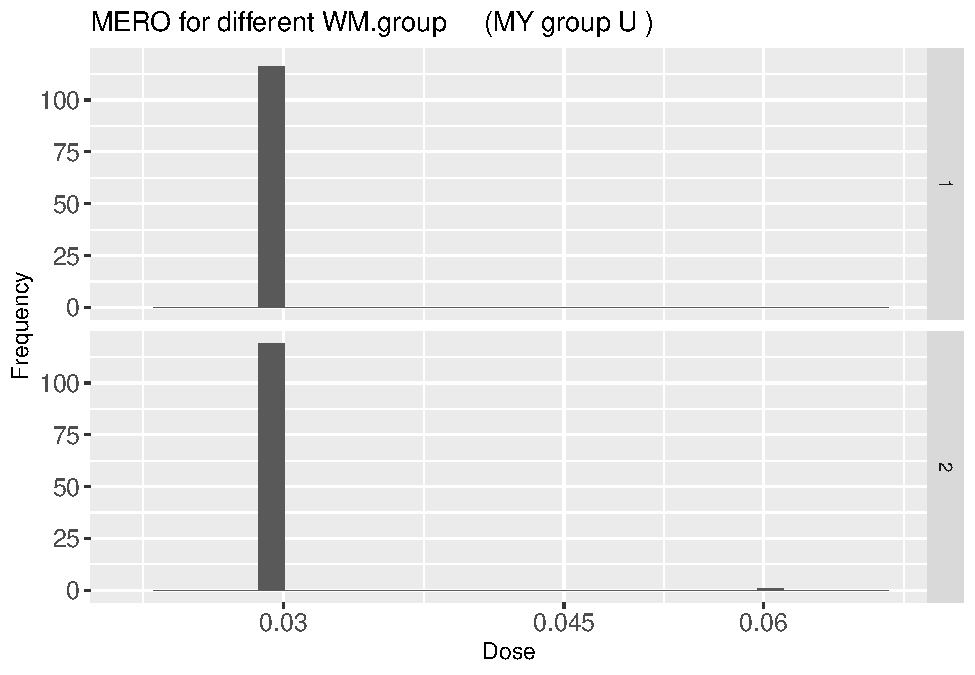
\includegraphics{Verteilungen_files/figure-latex/unnamed-chunk-32-1.pdf}

Der Mittelwert ist vergleichbar ohne WM (tatsächlich tendenziell minimal
höher - das ist leicht zu kontrollieren: MERO ist immer \textless=3 -
ausser einmal 0.06 für Betrieb 4 und der ist WM group 2).

\begin{Shaded}
\begin{Highlighting}[]
  \KeywordTok{graphisch}\NormalTok{(}\StringTok{"WM.group"}\NormalTok{, }\StringTok{"CIP"}\NormalTok{, }\FloatTok{0.015}\NormalTok{,}\DecValTok{8}\NormalTok{, }\FloatTok{.015}\NormalTok{,}\DecValTok{4}\NormalTok{) }
\end{Highlighting}
\end{Shaded}

\begin{verbatim}
## [1] "CIP - Resistance, WM            :"
## [1] "  Median             <= 0.015"
## [1] "  Mean   in  0.132 ... 0.145"
## [1] ""
## [1] "CIP - Resistance, no WM      :"
## [1] "  Median             <= 0.015"
## [1] "  Mean   in  0.577 ... 0.590"
## [1] ""
\end{verbatim}

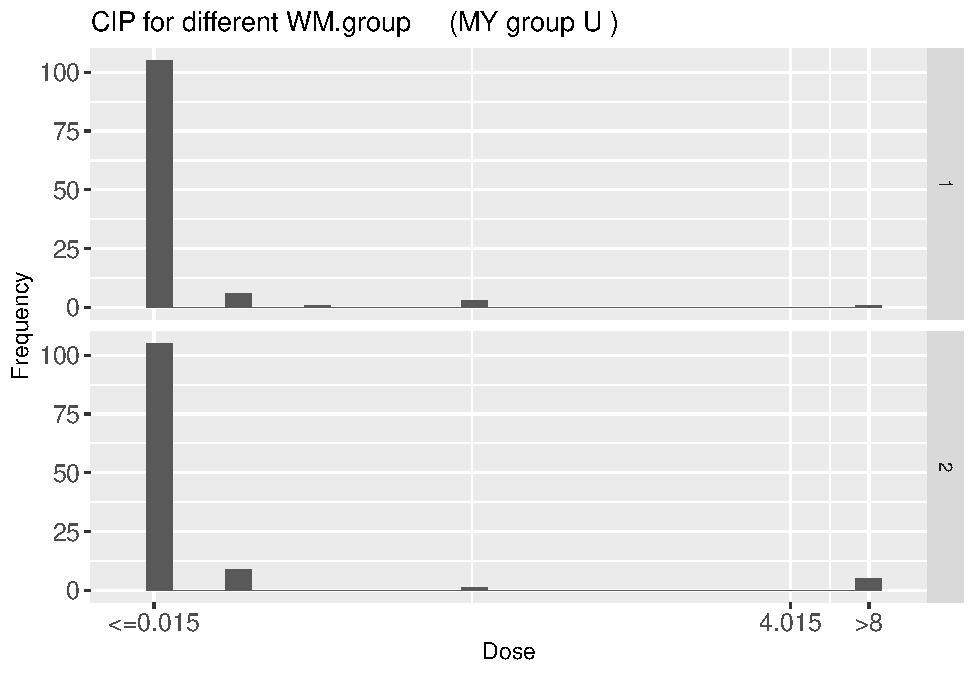
\includegraphics{Verteilungen_files/figure-latex/unnamed-chunk-33-1.pdf}

Der Mittelwert ist tendenziell höher ohne WM.

\begin{Shaded}
\begin{Highlighting}[]
  \KeywordTok{graphisch}\NormalTok{(}\StringTok{"WM.group"}\NormalTok{, }\StringTok{"AZI"}\NormalTok{, }\DecValTok{2}\NormalTok{,}\DecValTok{64}\NormalTok{, }\DecValTok{1}\NormalTok{,}\DecValTok{10}\NormalTok{)}
\end{Highlighting}
\end{Shaded}

\begin{verbatim}
## [1] "AZI - Resistance, WM            :"
## [1] "  Median             = 8"
## [1] "  Mean   in  6.812 ... 6.875"
## [1] ""
## [1] "AZI - Resistance, no WM      :"
## [1] "  Median             = 8"
## [1] "  Mean   in  7.643 ... 7.679"
## [1] ""
\end{verbatim}

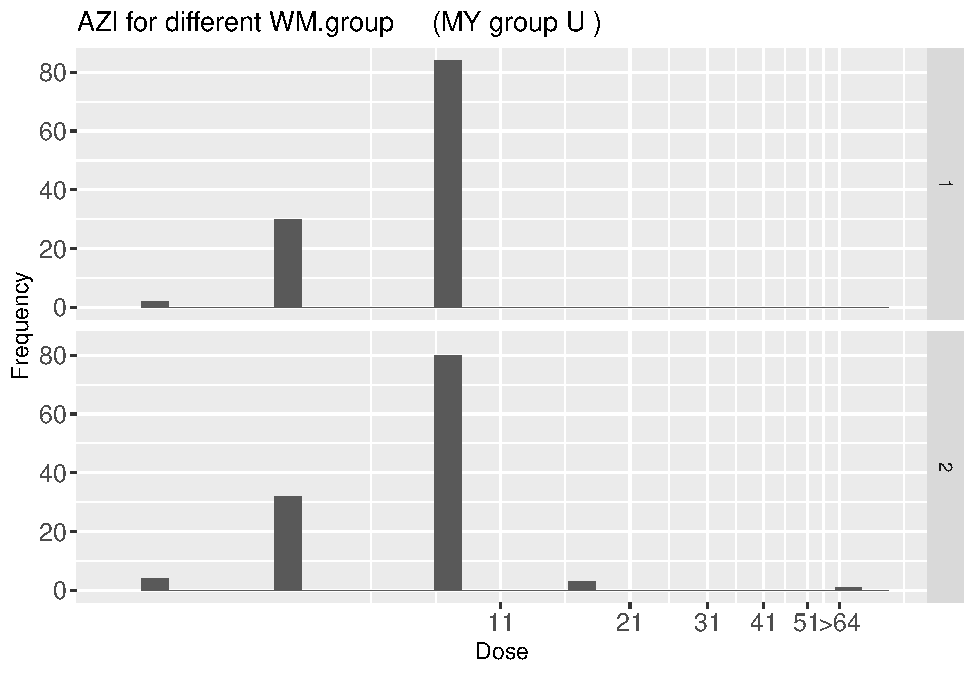
\includegraphics{Verteilungen_files/figure-latex/unnamed-chunk-34-1.pdf}

Der Mittelwert ist höher ohne WM.

\begin{Shaded}
\begin{Highlighting}[]
  \KeywordTok{graphisch}\NormalTok{(}\StringTok{"WM.group"}\NormalTok{, }\StringTok{"GEN"}\NormalTok{, }\FloatTok{0.5}\NormalTok{,}\DecValTok{16}\NormalTok{, }\FloatTok{0.5}\NormalTok{,}\DecValTok{4}\NormalTok{)}
\end{Highlighting}
\end{Shaded}

\begin{verbatim}
## [1] "GEN - Resistance, WM            :"
## [1] "  Median             <= 0.5"
## [1] "  Mean   in  0.984 ... 1.398"
## [1] ""
## [1] "GEN - Resistance, no WM      :"
## [1] "  Median             <= 0.5"
## [1] "  Mean   in  0.964 ... 1.375"
## [1] ""
\end{verbatim}

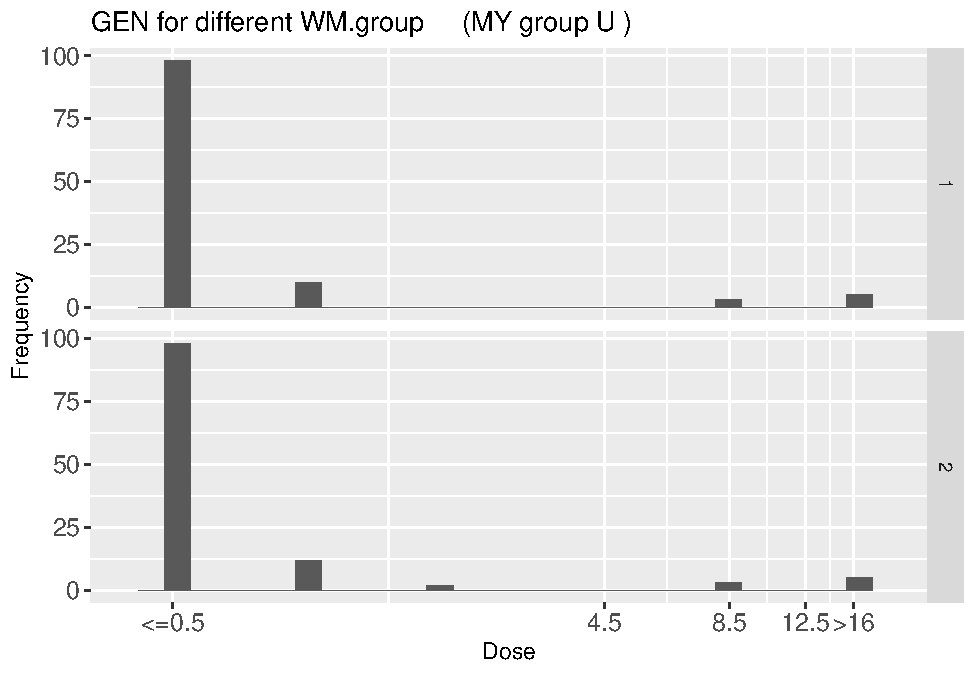
\includegraphics{Verteilungen_files/figure-latex/unnamed-chunk-35-1.pdf}

Der Mittelwert ist vergleichbar ohne WM.

\begin{Shaded}
\begin{Highlighting}[]
  \KeywordTok{graphisch}\NormalTok{(}\StringTok{"WM.group"}\NormalTok{, }\StringTok{"TGC"}\NormalTok{, }\FloatTok{0.25}\NormalTok{,}\OperatorTok{-}\FloatTok{0.5}\NormalTok{, }\FloatTok{0.25}\NormalTok{,}\FloatTok{0.25}\NormalTok{)  }
\end{Highlighting}
\end{Shaded}

\begin{verbatim}
## [1] "TGC - Resistance, WM            :"
## [1] "  Median             <= 0.25"
## [1] "  Mean   in  0.070 ... 0.285"
## [1] ""
## [1] "TGC - Resistance, no WM      :"
## [1] "  Median             <= 0.25"
## [1] "  Mean   in  0.054 ... 0.277"
## [1] ""
\end{verbatim}

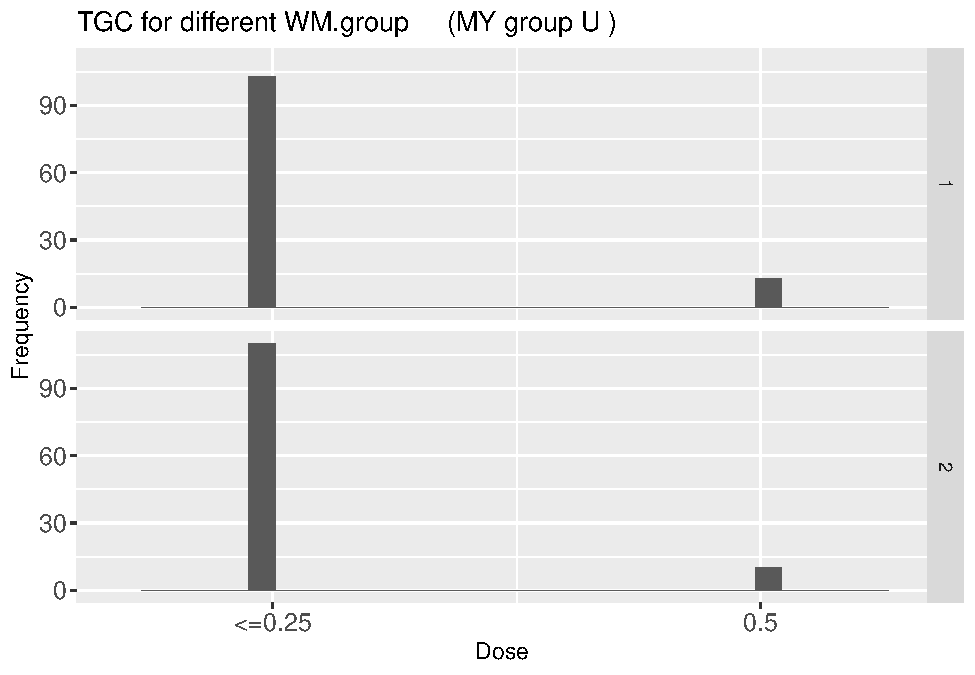
\includegraphics{Verteilungen_files/figure-latex/unnamed-chunk-36-1.pdf}

Der Mittelwert ist vergleichbar ohne WM.

\begin{Shaded}
\begin{Highlighting}[]
  \KeywordTok{graphisch}\NormalTok{(}\StringTok{"WM.group"}\NormalTok{, }\StringTok{"TAZ"}\NormalTok{, }\FloatTok{0.25}\NormalTok{, }\DecValTok{-1}\NormalTok{, }\FloatTok{.25}\NormalTok{,.}\DecValTok{25}\NormalTok{)  }
\end{Highlighting}
\end{Shaded}

\begin{verbatim}
## [1] "TAZ - Resistance, WM            :"
## [1] "  Median             <= 0.25"
## [1] "  Mean   in  0.000 ... 0.250"
## [1] ""
## [1] "TAZ - Resistance, no WM      :"
## [1] "  Median             <= 0.25"
## [1] "  Mean   in  0.062 ... 0.295"
## [1] ""
\end{verbatim}

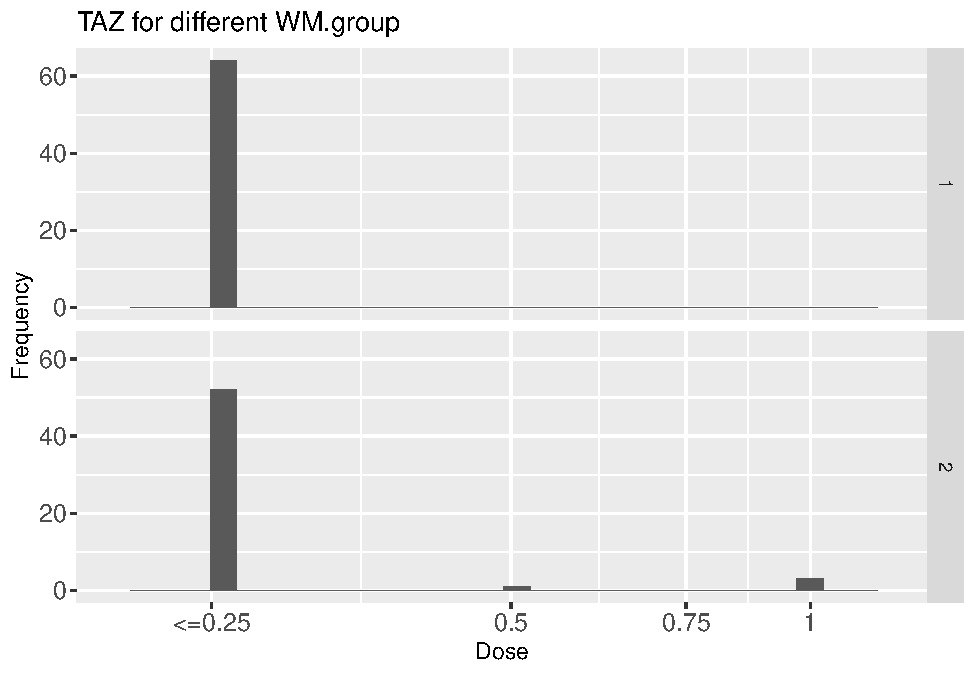
\includegraphics{Verteilungen_files/figure-latex/unnamed-chunk-37-1.pdf}

Der Mittelwert ist vergleichbar ohne WM. Genauer: tendenziell höher -
das kann man auch noch per Hand kontrollieren: TAZ ist immer \textless=
0.25 ausser für:

\begin{itemize}
\tightlist
\item
  Waste Milk: 0.5 für Betriebe 11 und 15
\item
  Keine Waste Milk: 0.5 für Betriebe 12, 59 und 3*1 für Betrieb 52
\end{itemize}

(Betrieb 30 wurde ganz am Anfang schon gelöscht)

Die Werte 0.5 balanzieren sich also aus für Waste Milk oder nicht, und
der Unterschied kommt von den 3 Werten 1: Ohne WM ist resistenter.

\begin{Shaded}
\begin{Highlighting}[]
  \KeywordTok{graphisch}\NormalTok{(}\StringTok{"WM.group"}\NormalTok{, }\StringTok{"FOT"}\NormalTok{, }\FloatTok{0.25}\NormalTok{,  }\DecValTok{4}\NormalTok{, }\FloatTok{.25}\NormalTok{, }\DecValTok{1}\NormalTok{)  }
\end{Highlighting}
\end{Shaded}

\begin{verbatim}
## [1] "FOT - Resistance, WM            :"
## [1] "  Median             <= 0.25"
## [1] "  Mean   in  0.000 ... 0.250"
## [1] ""
## [1] "FOT - Resistance, no WM      :"
## [1] "  Median             <= 0.25"
## [1] "  Mean   in  0.214 ... 0.451"
## [1] ""
\end{verbatim}

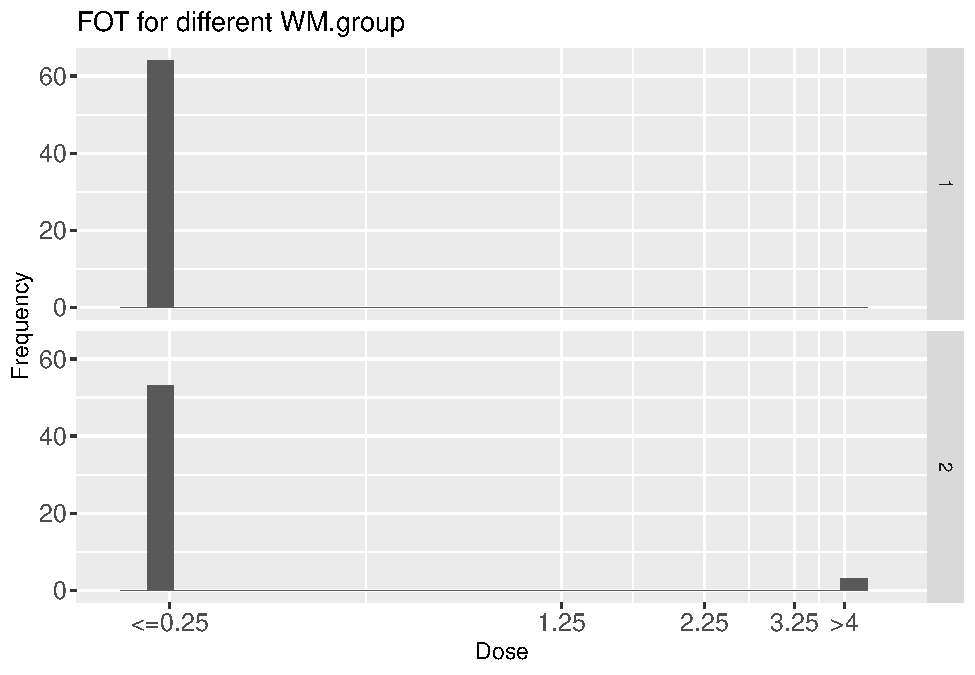
\includegraphics{Verteilungen_files/figure-latex/unnamed-chunk-38-1.pdf}

Der Mittelwert ist tendenziell höher ohne WM.

\begin{Shaded}
\begin{Highlighting}[]
  \KeywordTok{graphisch}\NormalTok{(}\StringTok{"WM.group"}\NormalTok{, }\StringTok{"CHL"}\NormalTok{, }\DecValTok{8}\NormalTok{,}\DecValTok{64}\NormalTok{, }\DecValTok{8}\NormalTok{,}\DecValTok{16}\NormalTok{) }
\end{Highlighting}
\end{Shaded}

\begin{verbatim}
## [1] "CHL - Resistance, WM            :"
## [1] "  Median             <= 8"
## [1] "  Mean   in  10.750 ... 17.125"
## [1] ""
## [1] "CHL - Resistance, no WM      :"
## [1] "  Median             <= 8"
## [1] "  Mean   in  16.571 ... 22.286"
## [1] ""
\end{verbatim}

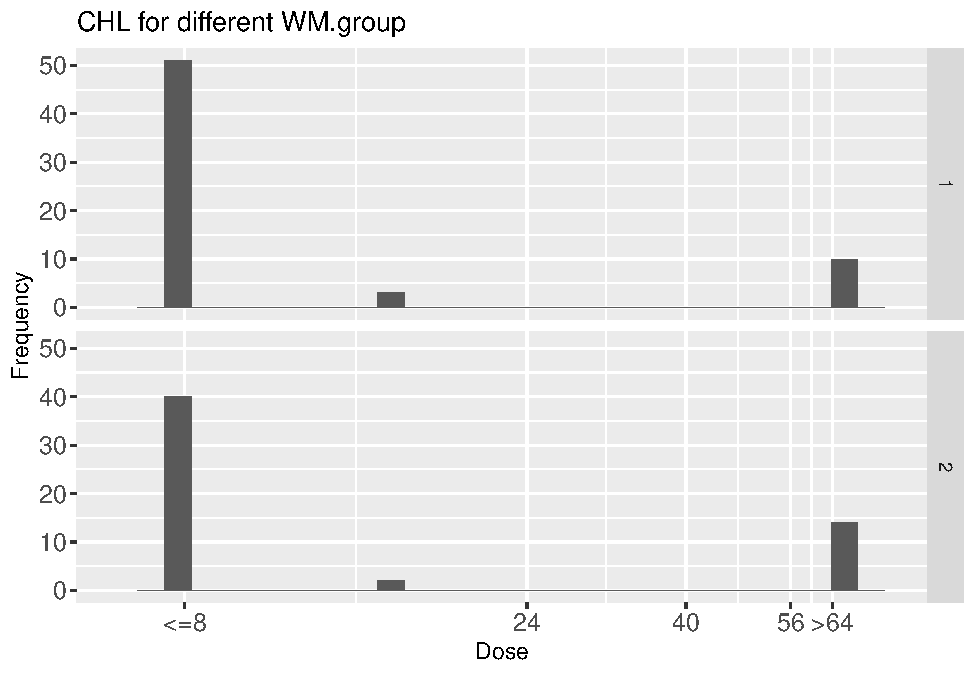
\includegraphics{Verteilungen_files/figure-latex/unnamed-chunk-39-1.pdf}

Der Mittelwert ist tendenziell höher ohne WM.

\begin{Shaded}
\begin{Highlighting}[]
  \KeywordTok{graphisch}\NormalTok{(}\StringTok{"WM.group"}\NormalTok{, }\StringTok{"NAL"}\NormalTok{, }\DecValTok{4}\NormalTok{,}\DecValTok{64}\NormalTok{, }\DecValTok{4}\NormalTok{,}\DecValTok{16}\NormalTok{) }
\end{Highlighting}
\end{Shaded}

\begin{verbatim}
## [1] "NAL - Resistance, WM            :"
## [1] "  Median             <= 4"
## [1] "  Mean   in  2.125 ... 5.938"
## [1] ""
## [1] "NAL - Resistance, no WM      :"
## [1] "  Median             <= 4"
## [1] "  Mean   in  4.857 ... 8.429"
## [1] ""
\end{verbatim}

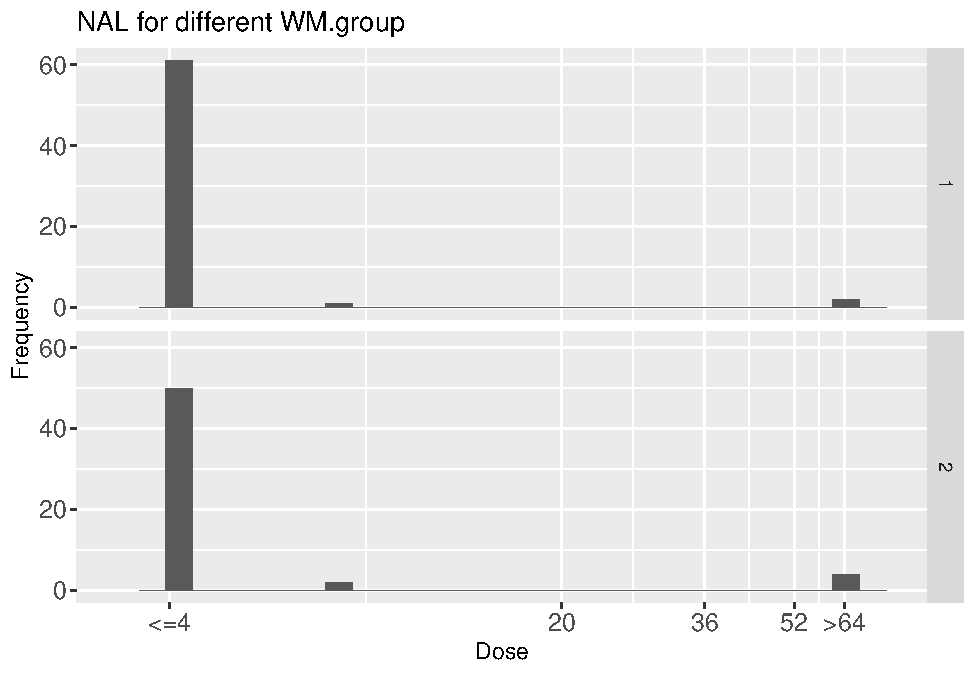
\includegraphics{Verteilungen_files/figure-latex/unnamed-chunk-40-1.pdf}

Der Mittelwert ist tendenziell höher ohne WM.

\begin{Shaded}
\begin{Highlighting}[]
  \KeywordTok{graphisch}\NormalTok{(}\StringTok{"WM.group"}\NormalTok{, }\StringTok{"TET"}\NormalTok{, }\DecValTok{2}\NormalTok{,}\DecValTok{32}\NormalTok{, }\DecValTok{2}\NormalTok{,}\DecValTok{8}\NormalTok{) }
\end{Highlighting}
\end{Shaded}

\begin{verbatim}
## [1] "TET - Resistance, WM            :"
## [1] "  Median             <= 2"
## [1] "  Mean   in  10.938 ... 12.062"
## [1] ""
## [1] "TET - Resistance, no WM      :"
## [1] "  Median             <= 2"
## [1] "  Mean   in  12.929 ... 14.000"
## [1] ""
\end{verbatim}

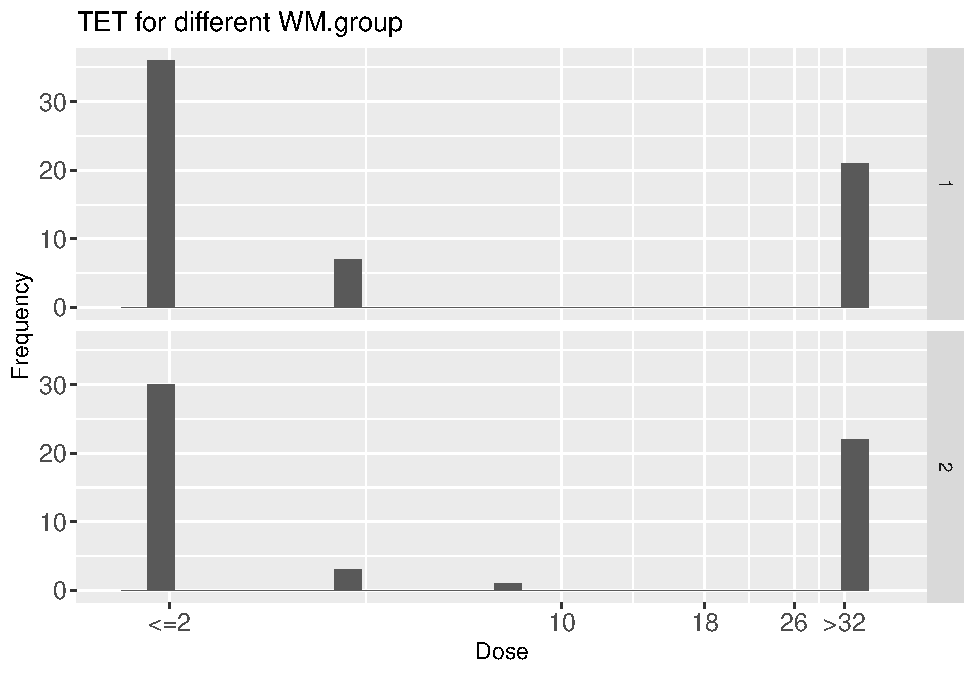
\includegraphics{Verteilungen_files/figure-latex/unnamed-chunk-41-1.pdf}

Der Mittelwert ist tendenziell höher ohne WM.

\begin{Shaded}
\begin{Highlighting}[]
  \KeywordTok{graphisch}\NormalTok{(}\StringTok{"WM.group"}\NormalTok{, }\StringTok{"TMP"}\NormalTok{, }\FloatTok{0.25}\NormalTok{,}\DecValTok{16}\NormalTok{, }\FloatTok{.25}\NormalTok{,}\DecValTok{8}\NormalTok{) }
\end{Highlighting}
\end{Shaded}

\begin{verbatim}
## [1] "TMP - Resistance, WM            :"
## [1] "  Median             = 0.5"
## [1] "  Mean   in  1.617 ... 1.672"
## [1] ""
## [1] "TMP - Resistance, no WM      :"
## [1] "  Median             = 0.5"
## [1] "  Mean   in  5.955 ... 6.004"
## [1] ""
\end{verbatim}

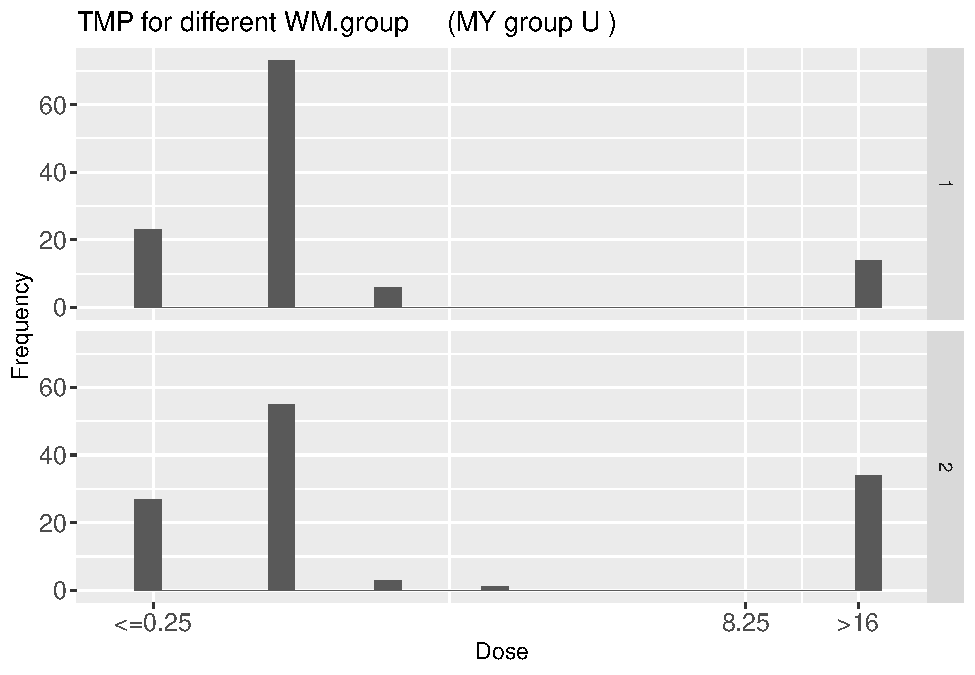
\includegraphics{Verteilungen_files/figure-latex/unnamed-chunk-42-1.pdf}

Der Mittelwert ist höher ohne WM.

\begin{Shaded}
\begin{Highlighting}[]
  \KeywordTok{graphisch}\NormalTok{(}\StringTok{"WM.group"}\NormalTok{, }\StringTok{"SMX"}\NormalTok{, }\DecValTok{8}\NormalTok{,}\DecValTok{512}\NormalTok{, }\DecValTok{8}\NormalTok{,}\DecValTok{256}\NormalTok{) }
\end{Highlighting}
\end{Shaded}

\begin{verbatim}
## [1] "SMX - Resistance, WM            :"
## [1] "  Median             = 16"
## [1] "  Mean   in  176.000 ... 178.000"
## [1] ""
## [1] "SMX - Resistance, no WM      :"
## [1] "  Median             = 32"
## [1] "  Mean   in  252.571 ... 254.429"
## [1] ""
\end{verbatim}

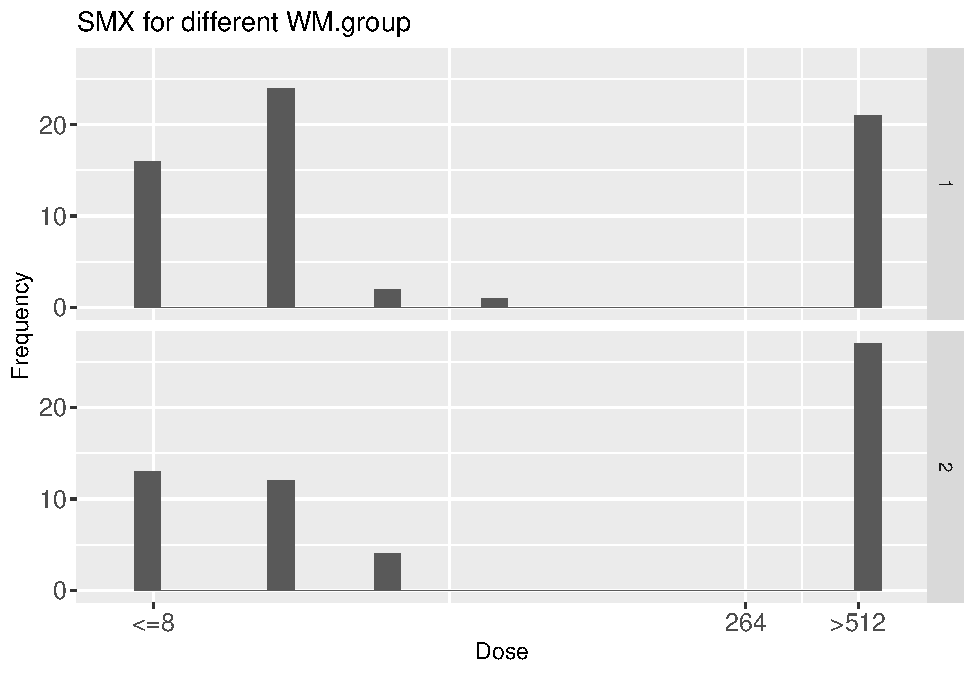
\includegraphics{Verteilungen_files/figure-latex/unnamed-chunk-43-1.pdf}

Der Mittelwert ist vergleichbar ohne WM.

Die Mittelwerte der Resistenz sind für 5 Antibiotika vergleichbar (MERO,
GEN, TGC, TAZ, SMX), für 3 Antibiotika tendenziell grösser im Fall
\emph{WM} (CIP, FOT, NAL) und für 5 Antibiotika definitiv grösser in
diesem Fall (AMP, AZI, HCL, TET, TMP).

\hypertarget{husbandry-system-calves---gruppen}{%
\section{Husbandry System Calves -
Gruppen}\label{husbandry-system-calves---gruppen}}

Mit ``HSC'' abgekürzt.

\begin{Shaded}
\begin{Highlighting}[]
  \KeywordTok{graphisch}\NormalTok{(}\StringTok{"HSC.group"}\NormalTok{, }\StringTok{"AMP"}\NormalTok{, }\DecValTok{1}\NormalTok{,}\DecValTok{32}\NormalTok{, }\DecValTok{1}\NormalTok{,}\DecValTok{8}\NormalTok{)}
\end{Highlighting}
\end{Shaded}

\begin{verbatim}
## [1] "AMP - Resistance, 0: stable w\\o  outlet :"
## [1] "  Median             = 4"
## [1] "  Mean   =  11.458"
## [1] ""
## [1] "AMP - Resistance, 1: stable with outlet :"
## [1] "  Median             = 4"
## [1] "  Mean   =  14.071"
## [1] ""
## [1] "AMP - Resistance, 2: outdoors           :"
## [1] "  Median             = 4"
## [1] "  Mean   =  12.000"
## [1] ""
## [1] "AMP - Resistance, 0+1                   :"
## [1] "  Median             = 4"
## [1] "  Mean   =  8.000"
## [1] ""
## [1] "AMP - Resistance, 1+2                   :"
## [1] "  Median             = 4"
## [1] "  Mean   =  13.000"
## [1] ""
## [1] "AMP - Resistance, 0+2                   :"
## [1] "  Median             = 18"
## [1] "  Mean   =  17.500"
## [1] ""
\end{verbatim}

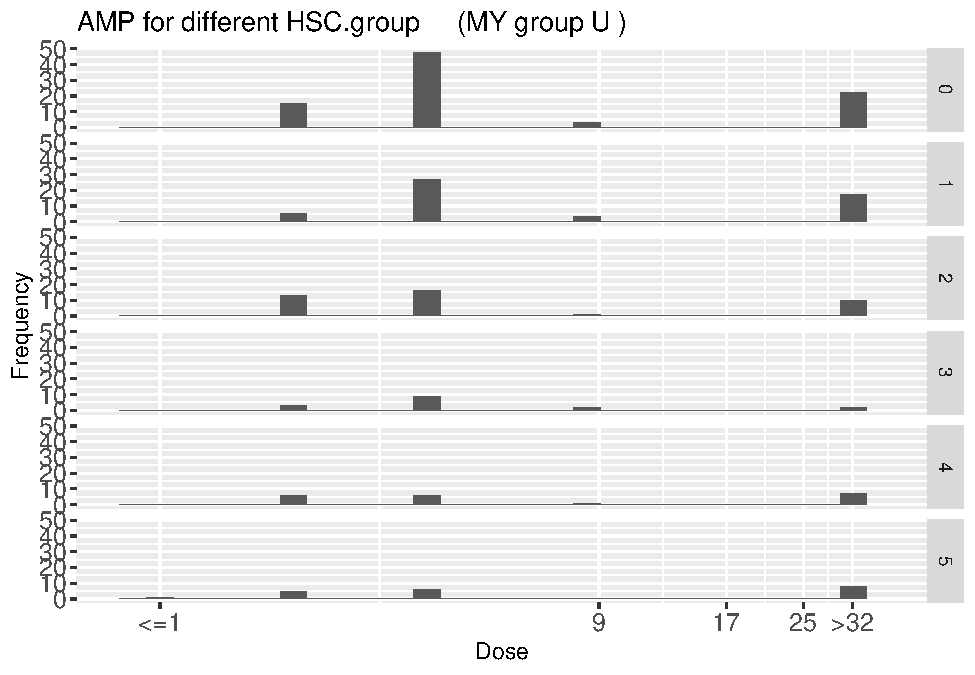
\includegraphics{Verteilungen_files/figure-latex/unnamed-chunk-44-1.pdf}

\begin{Shaded}
\begin{Highlighting}[]
  \KeywordTok{graphisch}\NormalTok{(}\StringTok{"HSC.group"}\NormalTok{, }\StringTok{"MERO"}\NormalTok{, }\FloatTok{0.03}\NormalTok{ ,  }\FloatTok{-0.06}\NormalTok{,   }\FloatTok{0.015}\NormalTok{,}\FloatTok{0.015}\NormalTok{)}
\end{Highlighting}
\end{Shaded}

\begin{verbatim}
## [1] "MERO - Resistance, 0: stable w\\o  outlet :"
## [1] "  Median             <= 0.03"
## [1] "  Mean   in  0.000 ... 0.030"
## [1] ""
## [1] "MERO - Resistance, 1: stable with outlet :"
## [1] "  Median             <= 0.03"
## [1] "  Mean   in  0.000 ... 0.030"
## [1] ""
## [1] "MERO - Resistance, 2: outdoors           :"
## [1] "  Median             <= 0.03"
## [1] "  Mean   in  0.000 ... 0.030"
## [1] ""
## [1] "MERO - Resistance, 0+1                   :"
## [1] "  Median             <= 0.03"
## [1] "  Mean   in  0.000 ... 0.030"
## [1] ""
## [1] "MERO - Resistance, 1+2                   :"
## [1] "  Median             <= 0.03"
## [1] "  Mean   in  0.000 ... 0.030"
## [1] ""
## [1] "MERO - Resistance, 0+2                   :"
## [1] "  Median             <= 0.03"
## [1] "  Mean   in  0.000 ... 0.030"
## [1] ""
\end{verbatim}

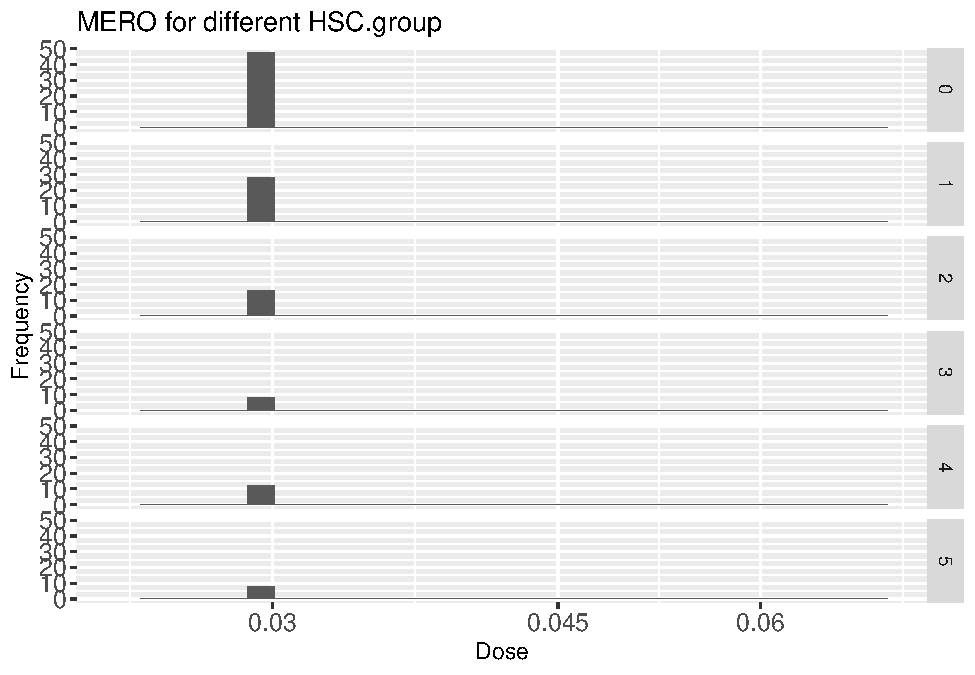
\includegraphics{Verteilungen_files/figure-latex/unnamed-chunk-45-1.pdf}

\begin{Shaded}
\begin{Highlighting}[]
  \KeywordTok{graphisch}\NormalTok{(}\StringTok{"HSC.group"}\NormalTok{, }\StringTok{"CIP"}\NormalTok{ , }\FloatTok{0.015}\NormalTok{,   }\DecValTok{8}\NormalTok{   ,   }\FloatTok{0.015}\NormalTok{,   }\DecValTok{4}\NormalTok{    ) }
\end{Highlighting}
\end{Shaded}

\begin{verbatim}
## [1] "CIP - Resistance, 0: stable w\\o  outlet :"
## [1] "  Median             <= 0.015"
## [1] "  Mean   in  0.508 ... 0.521"
## [1] ""
## [1] "CIP - Resistance, 1: stable with outlet :"
## [1] "  Median             <= 0.015"
## [1] "  Mean   in  0.010 ... 0.024"
## [1] ""
## [1] "CIP - Resistance, 2: outdoors           :"
## [1] "  Median             <= 0.015"
## [1] "  Mean   in  1.004 ... 1.015"
## [1] ""
## [1] "CIP - Resistance, 0+1                   :"
## [1] "  Median             <= 0.015"
## [1] "  Mean   in  0.000 ... 0.015"
## [1] ""
## [1] "CIP - Resistance, 1+2                   :"
## [1] "  Median             <= 0.015"
## [1] "  Mean   in  0.000 ... 0.015"
## [1] ""
## [1] "CIP - Resistance, 0+2                   :"
## [1] "  Median             <= 0.015"
## [1] "  Mean   in  0.004 ... 0.017"
## [1] ""
\end{verbatim}

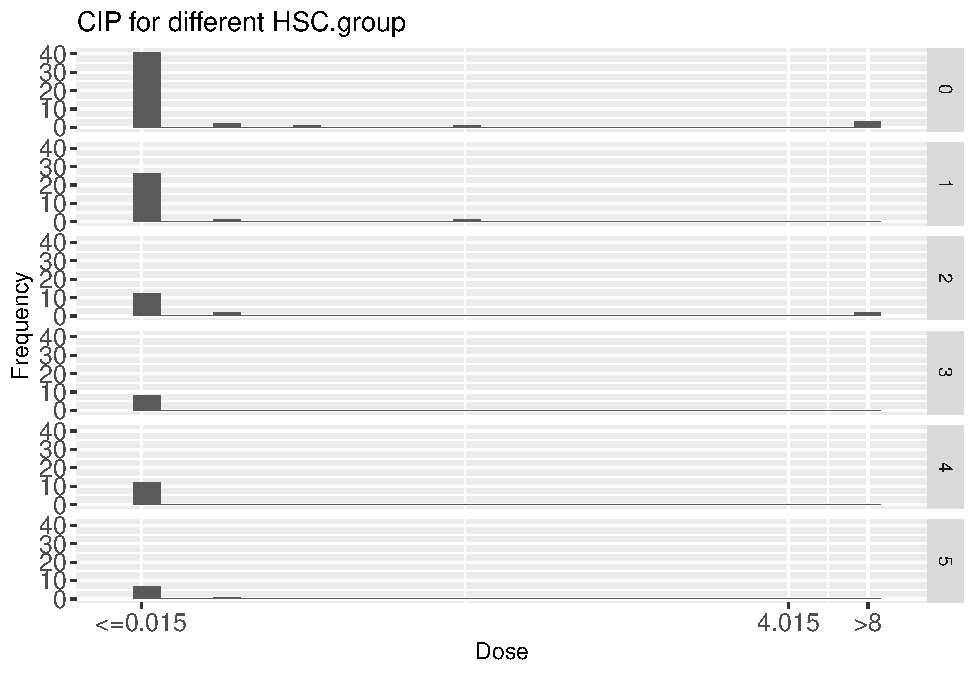
\includegraphics{Verteilungen_files/figure-latex/unnamed-chunk-46-1.pdf}

\begin{Shaded}
\begin{Highlighting}[]
   \KeywordTok{graphisch}\NormalTok{(}\StringTok{"HSC.group"}\NormalTok{, }\StringTok{"AZI"}\NormalTok{ , }\DecValTok{2}\NormalTok{    ,  }\DecValTok{64}\NormalTok{   ,   }\DecValTok{1}\NormalTok{    ,   }\DecValTok{10}\NormalTok{    )}
\end{Highlighting}
\end{Shaded}

\begin{verbatim}
## [1] "AZI - Resistance, 0: stable w\\o  outlet :"
## [1] "  Median             = 8"
## [1] "  Mean   =  8.000"
## [1] ""
## [1] "AZI - Resistance, 1: stable with outlet :"
## [1] "  Median             = 8"
## [1] "  Mean   in  6.286 ... 6.429"
## [1] ""
## [1] "AZI - Resistance, 2: outdoors           :"
## [1] "  Median             = 8"
## [1] "  Mean   =  7.000"
## [1] ""
## [1] "AZI - Resistance, 0+1                   :"
## [1] "  Median             = 8"
## [1] "  Mean   =  6.500"
## [1] ""
## [1] "AZI - Resistance, 1+2                   :"
## [1] "  Median             = 8"
## [1] "  Mean   in  7.667 ... 7.833"
## [1] ""
## [1] "AZI - Resistance, 0+2                   :"
## [1] "  Median             = 6"
## [1] "  Mean   =  6.000"
## [1] ""
\end{verbatim}

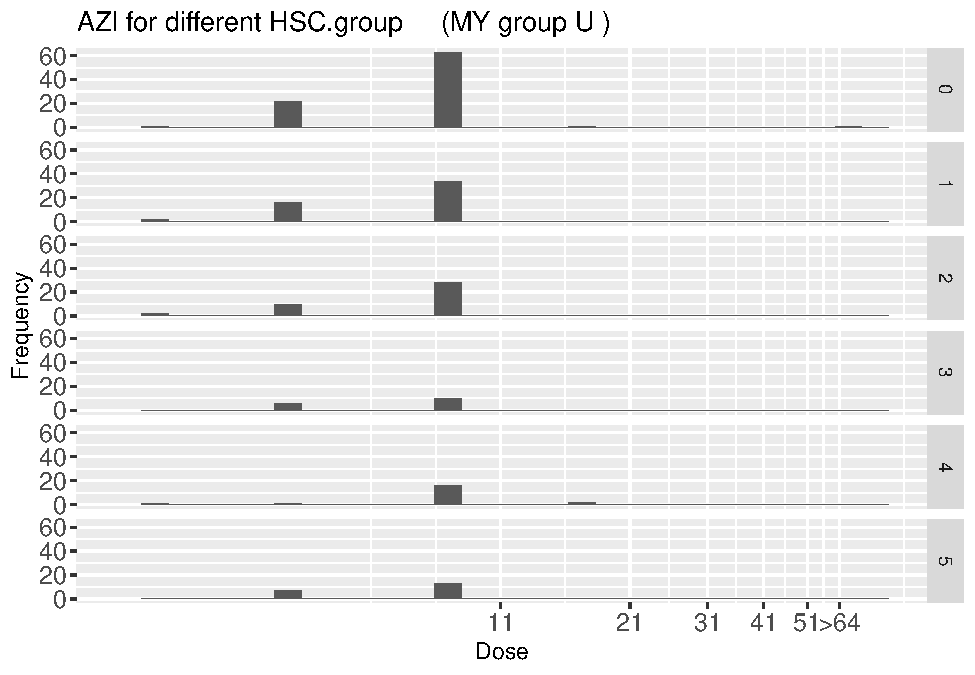
\includegraphics{Verteilungen_files/figure-latex/unnamed-chunk-47-1.pdf}

\begin{Shaded}
\begin{Highlighting}[]
   \KeywordTok{graphisch}\NormalTok{(}\StringTok{"HSC.group"}\NormalTok{, }\StringTok{"GEN"}\NormalTok{ , }\FloatTok{0.5}\NormalTok{  ,  }\DecValTok{16}\NormalTok{   ,   }\FloatTok{0.5}\NormalTok{  ,   }\DecValTok{4}\NormalTok{    )}
\end{Highlighting}
\end{Shaded}

\begin{verbatim}
## [1] "GEN - Resistance, 0: stable w\\o  outlet :"
## [1] "  Median             <= 0.5"
## [1] "  Mean   in  0.750 ... 1.177"
## [1] ""
## [1] "GEN - Resistance, 1: stable with outlet :"
## [1] "  Median             <= 0.5"
## [1] "  Mean   in  1.536 ... 1.929"
## [1] ""
## [1] "GEN - Resistance, 2: outdoors           :"
## [1] "  Median             <= 0.5"
## [1] "  Mean   in  2.188 ... 2.531"
## [1] ""
## [1] "GEN - Resistance, 0+1                   :"
## [1] "  Median             <= 0.5"
## [1] "  Mean   in  0.000 ... 0.500"
## [1] ""
## [1] "GEN - Resistance, 1+2                   :"
## [1] "  Median             <= 0.5"
## [1] "  Mean   in  0.083 ... 0.542"
## [1] ""
## [1] "GEN - Resistance, 0+2                   :"
## [1] "  Median             <= 0.5"
## [1] "  Mean   in  0.250 ... 0.625"
## [1] ""
\end{verbatim}

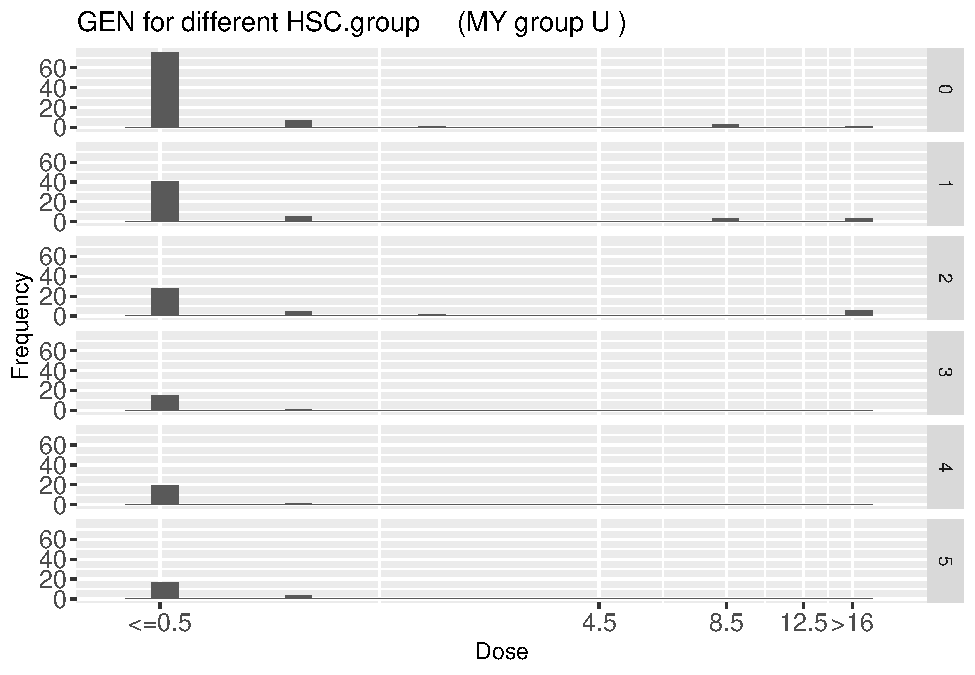
\includegraphics{Verteilungen_files/figure-latex/unnamed-chunk-48-1.pdf}

\begin{Shaded}
\begin{Highlighting}[]
   \KeywordTok{graphisch}\NormalTok{(}\StringTok{"HSC.group"}\NormalTok{, }\StringTok{"TGC"}\NormalTok{ , }\FloatTok{0.25}\NormalTok{ ,  }\FloatTok{-0.5}\NormalTok{ ,   }\FloatTok{0.25}\NormalTok{ ,   }\FloatTok{0.25}\NormalTok{ )  }
\end{Highlighting}
\end{Shaded}

\begin{verbatim}
## [1] "TGC - Resistance, 0: stable w\\o  outlet :"
## [1] "  Median             <= 0.25"
## [1] "  Mean   in  0.042 ... 0.271"
## [1] ""
## [1] "TGC - Resistance, 1: stable with outlet :"
## [1] "  Median             <= 0.25"
## [1] "  Mean   in  0.143 ... 0.321"
## [1] ""
## [1] "TGC - Resistance, 2: outdoors           :"
## [1] "  Median             <= 0.25"
## [1] "  Mean   in  0.031 ... 0.266"
## [1] ""
## [1] "TGC - Resistance, 0+1                   :"
## [1] "  Median             <= 0.25"
## [1] "  Mean   in  0.062 ... 0.281"
## [1] ""
## [1] "TGC - Resistance, 1+2                   :"
## [1] "  Median             <= 0.25"
## [1] "  Mean   in  0.042 ... 0.271"
## [1] ""
## [1] "TGC - Resistance, 0+2                   :"
## [1] "  Median             <= 0.25"
## [1] "  Mean   in  0.000 ... 0.250"
## [1] ""
\end{verbatim}

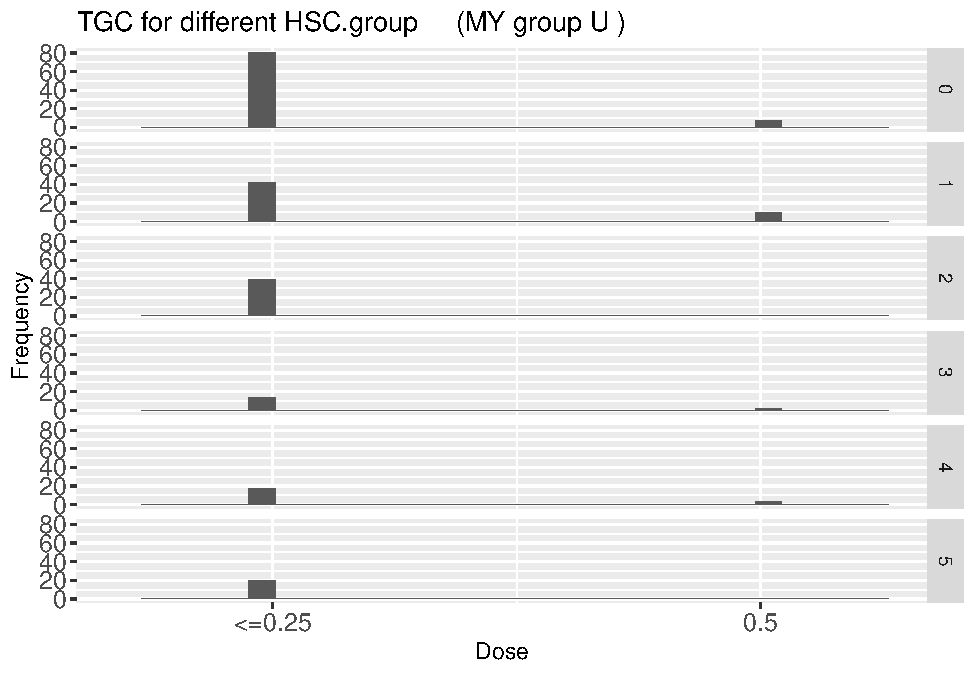
\includegraphics{Verteilungen_files/figure-latex/unnamed-chunk-49-1.pdf}

\begin{Shaded}
\begin{Highlighting}[]
   \KeywordTok{graphisch}\NormalTok{(}\StringTok{"HSC.group"}\NormalTok{, }\StringTok{"TAZ"}\NormalTok{ , }\FloatTok{0.25}\NormalTok{ ,  }\DecValTok{-1}\NormalTok{   ,   }\FloatTok{0.25}\NormalTok{ ,   }\FloatTok{0.25}\NormalTok{ )  }
\end{Highlighting}
\end{Shaded}

\begin{verbatim}
## [1] "TAZ - Resistance, 0: stable w\\o  outlet :"
## [1] "  Median             <= 0.25"
## [1] "  Mean   in  0.062 ... 0.297"
## [1] ""
## [1] "TAZ - Resistance, 1: stable with outlet :"
## [1] "  Median             <= 0.25"
## [1] "  Mean   in  0.000 ... 0.250"
## [1] ""
## [1] "TAZ - Resistance, 2: outdoors           :"
## [1] "  Median             <= 0.25"
## [1] "  Mean   in  0.000 ... 0.250"
## [1] ""
## [1] "TAZ - Resistance, 0+1                   :"
## [1] "  Median             <= 0.25"
## [1] "  Mean   in  0.000 ... 0.250"
## [1] ""
## [1] "TAZ - Resistance, 1+2                   :"
## [1] "  Median             <= 0.25"
## [1] "  Mean   in  0.042 ... 0.271"
## [1] ""
## [1] "TAZ - Resistance, 0+2                   :"
## [1] "  Median             <= 0.25"
## [1] "  Mean   in  0.000 ... 0.250"
## [1] ""
\end{verbatim}

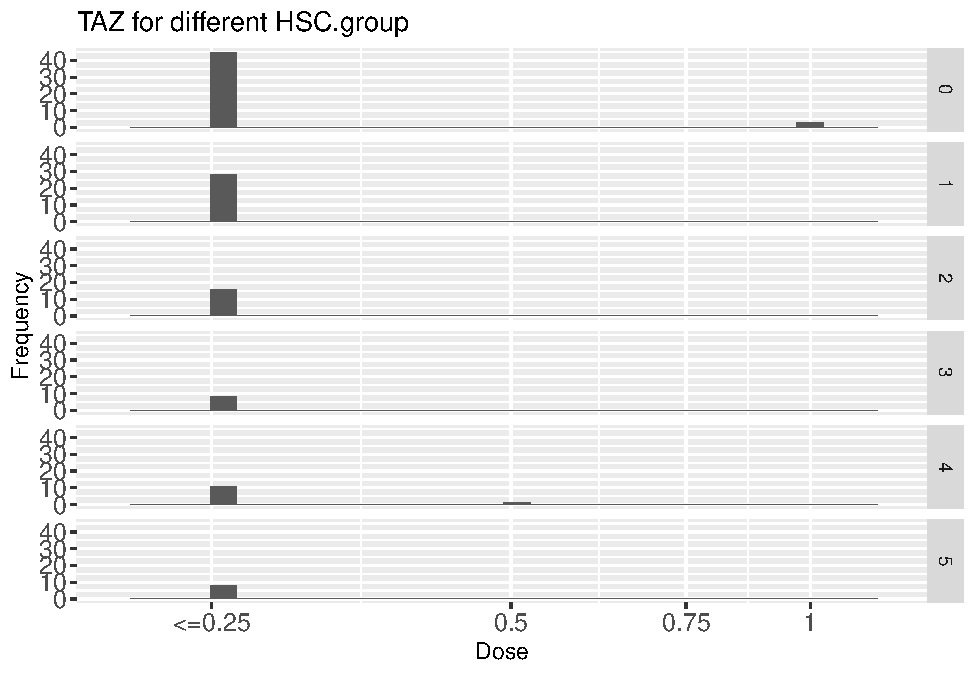
\includegraphics{Verteilungen_files/figure-latex/unnamed-chunk-50-1.pdf}

\begin{Shaded}
\begin{Highlighting}[]
  \KeywordTok{graphisch}\NormalTok{(}\StringTok{"HSC.group"}\NormalTok{, }\StringTok{"FOT"}\NormalTok{ , }\FloatTok{0.25}\NormalTok{ ,   }\DecValTok{4}\NormalTok{   ,   }\FloatTok{0.25}\NormalTok{ ,   }\DecValTok{1}\NormalTok{    )  }
\end{Highlighting}
\end{Shaded}

\begin{verbatim}
## [1] "FOT - Resistance, 0: stable w\\o  outlet :"
## [1] "  Median             <= 0.25"
## [1] "  Mean   in  0.250 ... 0.484"
## [1] ""
## [1] "FOT - Resistance, 1: stable with outlet :"
## [1] "  Median             <= 0.25"
## [1] "  Mean   in  0.000 ... 0.250"
## [1] ""
## [1] "FOT - Resistance, 2: outdoors           :"
## [1] "  Median             <= 0.25"
## [1] "  Mean   in  0.000 ... 0.250"
## [1] ""
## [1] "FOT - Resistance, 0+1                   :"
## [1] "  Median             <= 0.25"
## [1] "  Mean   in  0.000 ... 0.250"
## [1] ""
## [1] "FOT - Resistance, 1+2                   :"
## [1] "  Median             <= 0.25"
## [1] "  Mean   in  0.000 ... 0.250"
## [1] ""
## [1] "FOT - Resistance, 0+2                   :"
## [1] "  Median             <= 0.25"
## [1] "  Mean   in  0.000 ... 0.250"
## [1] ""
\end{verbatim}

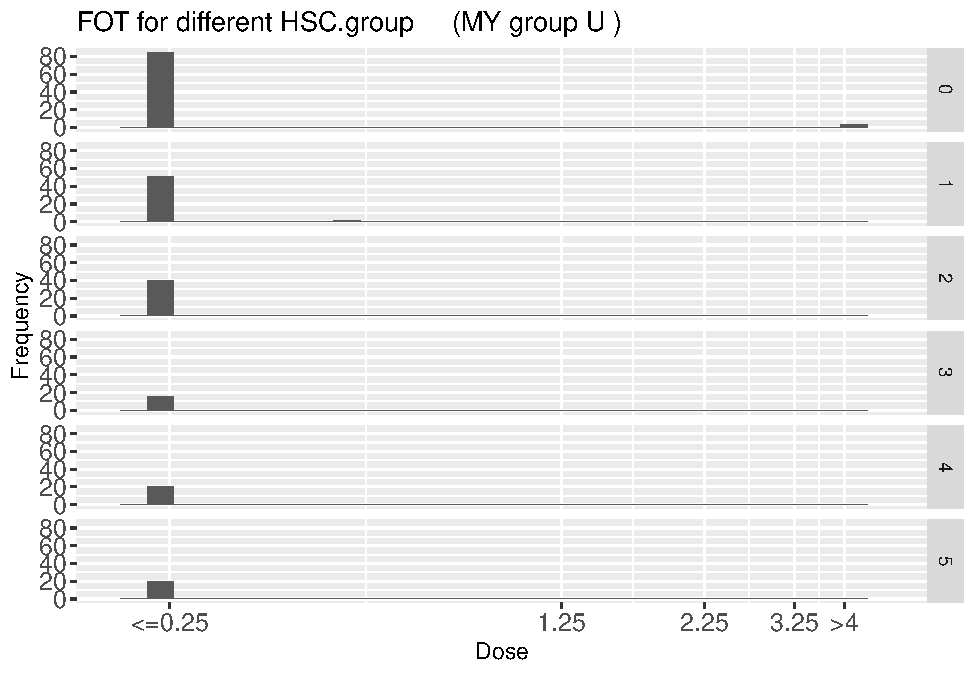
\includegraphics{Verteilungen_files/figure-latex/unnamed-chunk-51-1.pdf}

\begin{Shaded}
\begin{Highlighting}[]
   \KeywordTok{graphisch}\NormalTok{(}\StringTok{"HSC.group"}\NormalTok{, }\StringTok{"CHL"}\NormalTok{ , }\DecValTok{8}\NormalTok{    ,  }\DecValTok{64}\NormalTok{   ,   }\DecValTok{8}\NormalTok{,}\DecValTok{16}\NormalTok{   ) }
\end{Highlighting}
\end{Shaded}

\begin{verbatim}
## [1] "CHL - Resistance, 0: stable w\\o  outlet :"
## [1] "  Median             <= 8"
## [1] "  Mean   in  11.000 ... 17.500"
## [1] ""
## [1] "CHL - Resistance, 1: stable with outlet :"
## [1] "  Median             <= 8"
## [1] "  Mean   in  20.000 ... 24.857"
## [1] ""
## [1] "CHL - Resistance, 2: outdoors           :"
## [1] "  Median             <= 8"
## [1] "  Mean   in  12.000 ... 18.500"
## [1] ""
## [1] "CHL - Resistance, 0+1                   :"
## [1] "  Median             <= 8"
## [1] "  Mean   in  2.000 ... 9.000"
## [1] ""
## [1] "CHL - Resistance, 1+2                   :"
## [1] "  Median             <= 8"
## [1] "  Mean   in  5.333 ... 12.667"
## [1] ""
## [1] "CHL - Resistance, 0+2                   :"
## [1] "  Median             = 36"
## [1] "  Mean   in  32.000 ... 36.000"
## [1] ""
\end{verbatim}

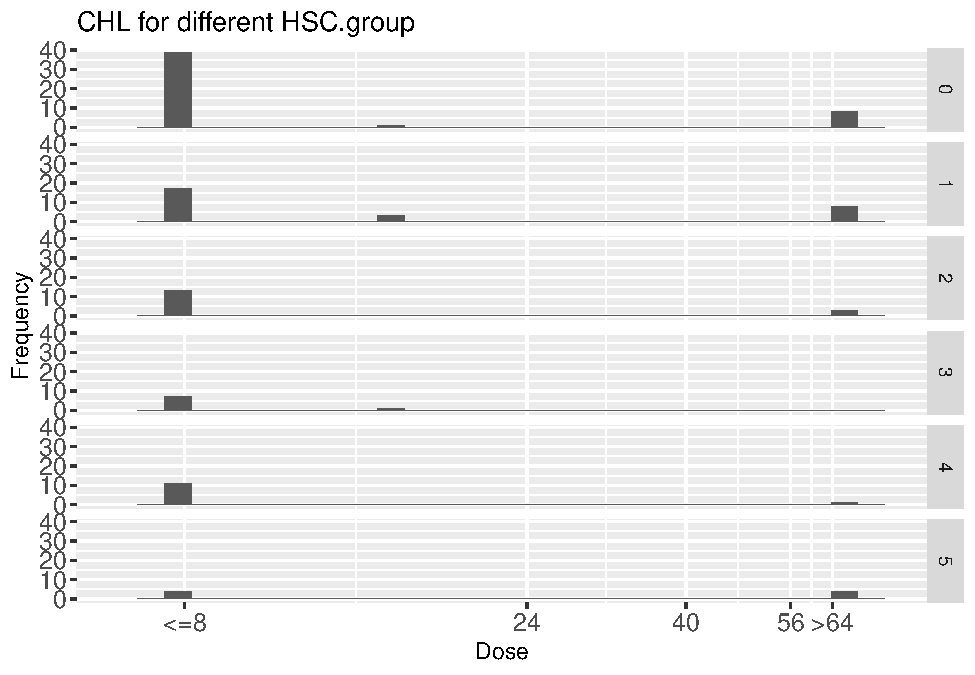
\includegraphics{Verteilungen_files/figure-latex/unnamed-chunk-52-1.pdf}

\begin{Shaded}
\begin{Highlighting}[]
   \KeywordTok{graphisch}\NormalTok{(}\StringTok{"HSC.group"}\NormalTok{, }\StringTok{"NAL"}\NormalTok{ , }\DecValTok{4}\NormalTok{    ,  }\DecValTok{64}\NormalTok{   ,   }\DecValTok{4}\NormalTok{,}\DecValTok{16}\NormalTok{   ) }
\end{Highlighting}
\end{Shaded}

\begin{verbatim}
## [1] "NAL - Resistance, 0: stable w\\o  outlet :"
## [1] "  Median             <= 4"
## [1] "  Mean   in  4.333 ... 7.917"
## [1] ""
## [1] "NAL - Resistance, 1: stable with outlet :"
## [1] "  Median             <= 4"
## [1] "  Mean   in  2.286 ... 6.143"
## [1] ""
## [1] "NAL - Resistance, 2: outdoors           :"
## [1] "  Median             <= 4"
## [1] "  Mean   in  8.000 ... 11.500"
## [1] ""
## [1] "NAL - Resistance, 0+1                   :"
## [1] "  Median             <= 4"
## [1] "  Mean   in  0.000 ... 4.000"
## [1] ""
## [1] "NAL - Resistance, 1+2                   :"
## [1] "  Median             <= 4"
## [1] "  Mean   in  0.000 ... 4.000"
## [1] ""
## [1] "NAL - Resistance, 0+2                   :"
## [1] "  Median             <= 4"
## [1] "  Mean   in  1.000 ... 4.500"
## [1] ""
\end{verbatim}

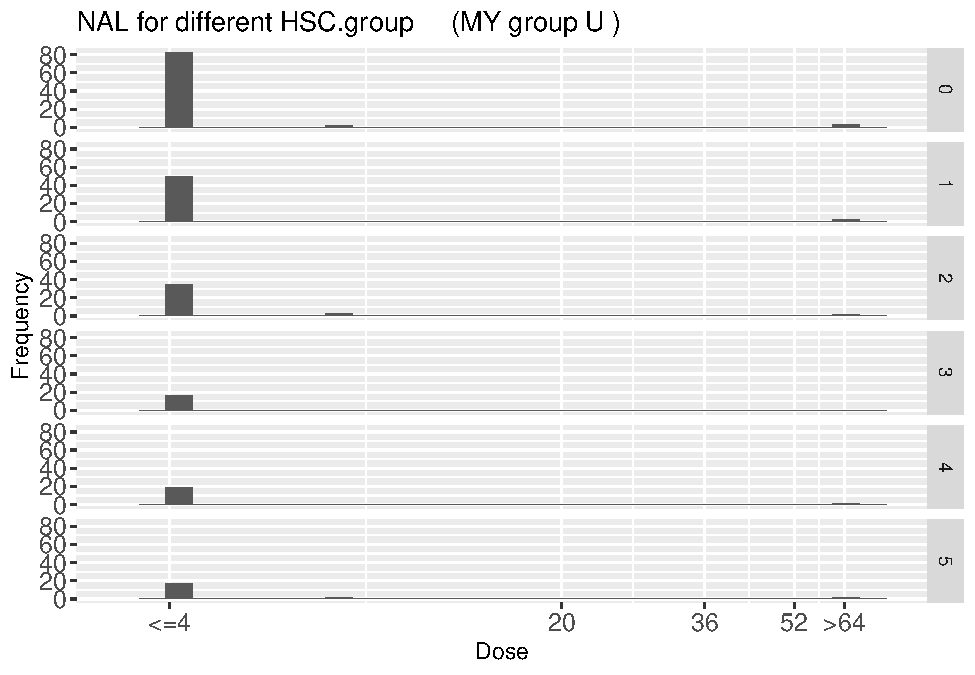
\includegraphics{Verteilungen_files/figure-latex/unnamed-chunk-53-1.pdf}

\begin{Shaded}
\begin{Highlighting}[]
   \KeywordTok{graphisch}\NormalTok{(}\StringTok{"HSC.group"}\NormalTok{, }\StringTok{"TET"}\NormalTok{ , }\DecValTok{2}\NormalTok{    ,  }\DecValTok{32}\NormalTok{   ,   }\DecValTok{2}\NormalTok{,}\DecValTok{8}\NormalTok{    ) }
\end{Highlighting}
\end{Shaded}

\begin{verbatim}
## [1] "TET - Resistance, 0: stable w\\o  outlet :"
## [1] "  Median             <= 2"
## [1] "  Mean   in  10.250 ... 11.500"
## [1] ""
## [1] "TET - Resistance, 1: stable with outlet :"
## [1] "  Median             = 4"
## [1] "  Mean   in  12.143 ... 13.071"
## [1] ""
## [1] "TET - Resistance, 2: outdoors           :"
## [1] "  Median             <= 2"
## [1] "  Mean   in  12.500 ... 13.625"
## [1] ""
## [1] "TET - Resistance, 0+1                   :"
## [1] "  Median             > 32"
## [1] "  Mean   in  20.000 ... 20.750"
## [1] ""
## [1] "TET - Resistance, 1+2                   :"
## [1] "  Median             <= 2"
## [1] "  Mean   in  8.667 ... 9.833"
## [1] ""
## [1] "TET - Resistance, 0+2                   :"
## [1] "  Median             = 17"
## [1] "  Mean   in  16.000 ... 17.000"
## [1] ""
\end{verbatim}

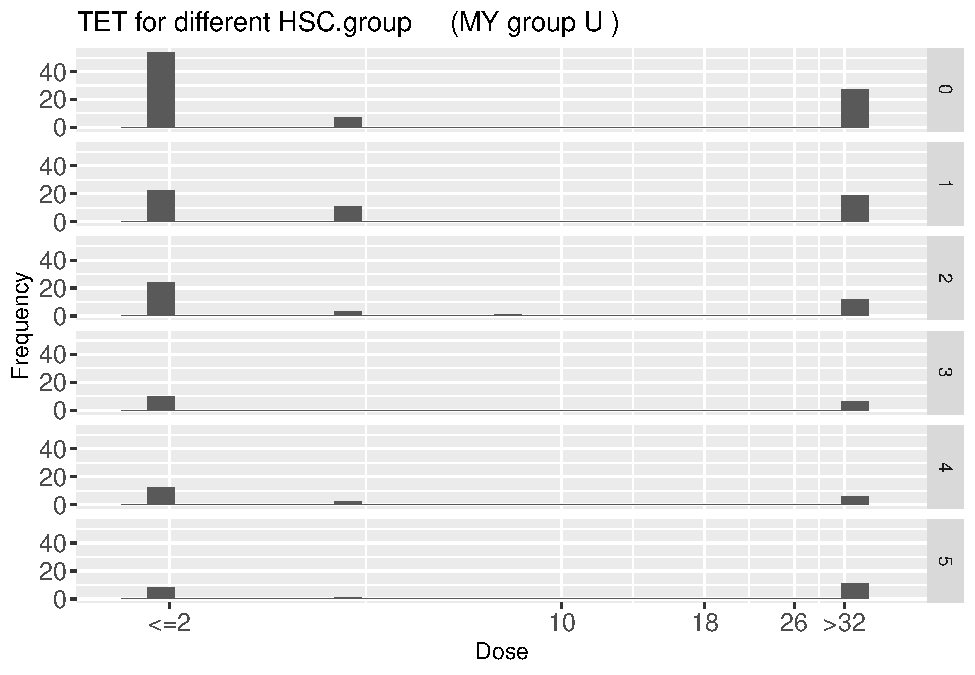
\includegraphics{Verteilungen_files/figure-latex/unnamed-chunk-54-1.pdf}

\begin{Shaded}
\begin{Highlighting}[]
   \KeywordTok{graphisch}\NormalTok{(}\StringTok{"HSC.group"}\NormalTok{, }\StringTok{"TMP"}\NormalTok{ , }\FloatTok{0.25}\NormalTok{ ,  }\DecValTok{16}\NormalTok{   ,   }\FloatTok{0.25}\NormalTok{,}\DecValTok{8}\NormalTok{    ) }
\end{Highlighting}
\end{Shaded}

\begin{verbatim}
## [1] "TMP - Resistance, 0: stable w\\o  outlet :"
## [1] "  Median             = 0.5"
## [1] "  Mean   in  3.958 ... 4.010"
## [1] ""
## [1] "TMP - Resistance, 1: stable with outlet :"
## [1] "  Median             = 0.5"
## [1] "  Mean   in  3.714 ... 3.768"
## [1] ""
## [1] "TMP - Resistance, 2: outdoors           :"
## [1] "  Median             = 0.5"
## [1] "  Mean   =  4.375"
## [1] ""
## [1] "TMP - Resistance, 0+1                   :"
## [1] "  Median             = 0.5"
## [1] "  Mean   in  0.500 ... 0.531"
## [1] ""
## [1] "TMP - Resistance, 1+2                   :"
## [1] "  Median             = 0.75"
## [1] "  Mean   in  5.667 ... 5.708"
## [1] ""
## [1] "TMP - Resistance, 0+2                   :"
## [1] "  Median             <= 0.25"
## [1] "  Mean   in  0.125 ... 0.312"
## [1] ""
\end{verbatim}

\includegraphics{Verteilungen_files/figure-latex/unnamed-chunk-55-1.pdf}

\begin{Shaded}
\begin{Highlighting}[]
  \KeywordTok{graphisch}\NormalTok{(}\StringTok{"HSC.group"}\NormalTok{, }\StringTok{"SMX"}\NormalTok{ , }\DecValTok{8}\NormalTok{    , }\DecValTok{512}\NormalTok{   ,   }\DecValTok{8}\NormalTok{,}\DecValTok{256}\NormalTok{    ) }
\end{Highlighting}
\end{Shaded}

\begin{verbatim}
## [1] "SMX - Resistance, 0: stable w\\o  outlet :"
## [1] "  Median             = 16"
## [1] "  Mean   in  198.667 ... 200.833"
## [1] ""
## [1] "SMX - Resistance, 1: stable with outlet :"
## [1] "  Median             = 16"
## [1] "  Mean   in  189.143 ... 191.429"
## [1] ""
## [1] "SMX - Resistance, 2: outdoors           :"
## [1] "  Median             = 24"
## [1] "  Mean   in  202.000 ... 203.000"
## [1] ""
## [1] "SMX - Resistance, 0+1                   :"
## [1] "  Median             > 512"
## [1] "  Mean   in  324.000 ... 325.000"
## [1] ""
## [1] "SMX - Resistance, 1+2                   :"
## [1] "  Median             = 32"
## [1] "  Mean   in  225.333 ... 226.000"
## [1] ""
## [1] "SMX - Resistance, 0+2                   :"
## [1] "  Median             = 260"
## [1] "  Mean   in  256.000 ... 260.000"
## [1] ""
\end{verbatim}

\includegraphics{Verteilungen_files/figure-latex/unnamed-chunk-56-1.pdf}

Es ist kein sehr ausgeprägtes Muster für grösste/kleinste Resistenzen zu
erkennen. Tendenziell ergeben 1 und 1+2 die grössten Resistenzen, 2 und
vor allem 0+1 die kleinsten.

\hypertarget{vollstuxe4ndigkeit}{%
\section{Vollständigkeit}\label{vollstuxe4ndigkeit}}

Jetzt sind alle Verteilungen geplotted und deskriptiv analysiert,
ausser:

\begin{itemize}
\tightlist
\item
  AMI: alle Proben sensitiv \textless=4
\item
  COL: alle Proben sensitiv \textless=1
\end{itemize}

\hypertarget{weitere-schritte}{%
\section{Weitere Schritte}\label{weitere-schritte}}

\hypertarget{technischer-natur}{%
\subsection{Technischer Natur}\label{technischer-natur}}

\begin{itemize}
\tightlist
\item
  noch minimale Verbesserungen Verteilungsplots?
\end{itemize}

\hypertarget{fundamentaler-natur}{%
\subsection{Fundamentaler Natur}\label{fundamentaler-natur}}

Kausalitäten studieren mittels Regressionen :

\begin{itemize}
\tightlist
\item
  Kausalitätsgraph
\item
  Lineare Regressionen?
\item
  multivariable logistische Regression \ldots{} mixed effects?
\end{itemize}

\newpage

\begin{itemize}
\tightlist
\item
  vs Assoziation:

  \begin{itemize}
  \tightlist
  \item
    Vorlesung Christian: ``Kausalität nur wenn immer der Fall''-!?
  \item
    Buch Scutari: ??
  \end{itemize}
\end{itemize}

\end{document}
